%Version 3.1 December 2024
% See section 11 of the User Manual for version history
%%%%%%%%%%%%%%%%%%%%%%%%%%%%%%%%%%%%%%%%%%%%%%%%%%%%%%%%%%%%%%%%%%%%%%
%%                                                                 %%
%% Please do not use \input{...} to include other tex files.       %%
%% Submit your LaTeX manuscript as one .tex document.              %%
%%                                                                 %%
%% All additional figures and files should be attached             %%
%% separately and not embedded in the \TeX\ document itself.       %%
%%                                                                 %%
%%%%%%%%%%%%%%%%%%%%%%%%%%%%%%%%%%%%%%%%%%%%%%%%%%%%%%%%%%%%%%%%%%%%%

%%\documentclass[referee,sn-basic]{sn-jnl}% referee option is meant for double line spacing

%%=======================================================%%
%% to print line numbers in the margin use lineno option %%
%%=======================================================%%

%%\documentclass[lineno,pdflatex,sn-basic]{sn-jnl}% Basic Springer Nature Reference Style/Chemistry Reference Style

%%=========================================================================================%%
%% the documentclass is set to pdflatex as default. You can delete it if not appropriate.  %%
%%=========================================================================================%%

%%\documentclass[sn-basic]{sn-jnl}% Basic Springer Nature Reference Style/Chemistry Reference Style

%%Note: the following reference styles support Namedate and Numbered referencing. By default the style follows the most common style. To switch between the options you can add or remove �Numbered� in the optional parenthesis.
%%The option is available for: sn-basic.bst, sn-chicago.bst%

\documentclass[pdflatex,sn-nature]{sn-jnl}% Style for submissions to Nature Portfolio journals
%\documentclass[pdflatex,sn-basic]{sn-jnl}% Basic Springer Nature Reference Style/Chemistry Reference Style
%\documentclass[pdflatex,sn-mathphys-num]{sn-jnl}% Math and Physical Sciences Numbered Reference Style
%\documentclass[pdflatex,sn-mathphys-ay]{sn-jnl}% Math and Physical Sciences Author Year Reference Style
%\documentclass[pdflatex,sn-aps]{sn-jnl}% American Physical Society (APS) Reference Style
%\documentclass[pdflatex,sn-vancouver-num]{sn-jnl}% Vancouver Numbered Reference Style
%\documentclass[pdflatex,sn-vancouver-ay]{sn-jnl}% Vancouver Author Year Reference Style
%\documentclass[pdflatex,sn-apa]{sn-jnl}% APA Reference Style
%\documentclass[pdflatex,sn-chicago]{sn-jnl}% Chicago-based Humanities Reference Style

%%%% Standard Packages
%%<additional latex packages if required can be included here>

\usepackage{graphicx}%
\usepackage{multirow}%
\usepackage{amsmath,amssymb,amsfonts}%
\usepackage{amsthm}%
\usepackage{mathrsfs}%
\usepackage[title]{appendix}%
\usepackage{xcolor}%
\usepackage{textcomp}%

% Define argmax operator
\DeclareMathOperator*{\argmax}{argmax}
\usepackage{manyfoot}%
\usepackage{booktabs}%
\usepackage{algorithm}%
\usepackage{algorithmicx}%
\usepackage{algpseudocode}%
\usepackage{listings}%

% \usepackage{caption}
\usepackage{standalone}
\usepackage{tikz}
\usepackage[dvipsnames]{xcolor}
\usepackage{geometry}
\usepackage{textcomp} % using \textquotesingle
% Minted package for beautiful syntax highlighting
\usepackage{minted}
\usemintedstyle{borland}
\setminted{
  fontsize=\small,
  breaklines=true,
  autogobble,
  frame=single,
  framesep=2mm,
  linenos
}

% Use bash lexer for TSG code examples (since it handles # comments well)
\newminted{bash}{
  fontsize=\small,
  breaklines=true,
  autogobble,
  frame=single,
  framesep=2mm,
  linenos
}

\usetikzlibrary{shadows,shapes,arrows,positioning,fit,backgrounds,decorations.pathreplacing,calc}

\graphicspath{{../figures}}

\usepackage[acronym, automake, style=index, shortcuts]{glossaries-extra}
\setabbreviationstyle[acronym]{long-short}
% define glossaries
\makeglossaries

\newacronym{wga}{WGA}{Whole Genome Amplification}
\newacronym{mda}{MDA}{Multiple Displacement Amplification}
\newacronym{malbac}{MALBAC}{Multiple Annealing and Looping-based Amplification Cycles}
\newacronym{gpu}{GPU}{Graphics Processing Unit}
\newacronym{cpu}{CPU}{Central Processing Unit}
\newacronym{hpc}{HPC}{High Performance Computing}
\newacronym{sv}{SV}{Structural Variation}
\newacronym{snp}{SNP}{Single Nucleotide Polymorphism}
\newacronym{ont}{ONT}{Oxford Nanopore Technologies}
\newacronym{pb}{PacBio}{Pacific Biosciences}
\newacronym{del}{DEL}{deletion}
\newacronym{dup}{DUP}{duplication}
\newacronym{ins}{INS}{insertion}
\newacronym{inv}{INV}{inversion}
\newacronym{tra}{TRA}{translocation}
\newacronym{pcr}{PCR}{Polymerase Chain Reaction}
\newacronym{mrna}{mRNA}{messenger RNA}
\newacronym{facs}{FACS}{Fluorescence-activated cell sorting}
\newacronym{sa}{SA}{Supplementary Alignment}
\newacronym{lianti}{LIANTI}{Linear Amplification via Transposon Insertion}
\newacronym{doppcr}{DOP-PCR}{termed Degenerate Oligonucleotide-Primed PCR}
\newacronym{pta}{PTA}{Primary Template-directed Amplification}
\newacronym{dmda}{dMDA}{droplet-based MDA}

\newacronym{ide}{IDE}{Integrated Development Environment}
\newacronym{cd}{CD}{Continuous Development}
\newacronym{ucsc}{UCSC}{UCSC Genome Browser}

\newacronym{glm}{GLM}{Genomic Language Model}
\newacronym{lcglm}{LCGLM}{long-context genomic language model}
\newacronym{mlp}{MLP}{multilayer perceptron}
\newacronym{gelu}{GELU}{Gaussian Error Linear Unit}

%%%%%=============================================================================%%%%
%%%%  Remarks: This template is provided to aid authors with the preparation
%%%%  of original research articles intended for submission to journals published
%%%%  by Springer Nature. The guidance has been prepared in partnership with
%%%%  production teams to conform to Springer Nature technical requirements.
%%%%  Editorial and presentation requirements differ among journal portfolios and
%%%%  research disciplines. You may find sections in this template are irrelevant
%%%%  to your work and are empowered to omit any such section if allowed by the
%%%%  journal you intend to submit to. The submission guidelines and policies
%%%%  of the journal take precedence. A detailed User Manual is available in the
%%%%  template package for technical guidance.
%%%%%=============================================================================%%%%

%% as per the requirement new theorem styles can be included as shown below
\theoremstyle{thmstyleone}%
\newtheorem{theorem}{Theorem}%  meant for continuous numbers
%%\newtheorem{theorem}{Theorem}[section]% meant for sectionwise numbers
%% optional argument [theorem] produces theorem numbering sequence instead of independent numbers for Proposition
\newtheorem{proposition}[theorem]{Proposition}%
%%\newtheorem{proposition}{Proposition}% to get separate numbers for theorem and proposition etc.

\theoremstyle{thmstyletwo}%
\newtheorem{example}{Example}%
\newtheorem{remark}{Remark}%

\theoremstyle{thmstylethree}%
\newtheorem{definition}{Definition}%

\raggedbottom
%%\unnumbered% uncomment this for unnumbered level heads

\begin{document}

\title[Article Title]{ChimeraLM detects amplification artifacts for accurate structural variant calling in long-read single-cell sequencing}

%%=============================================================%%
%% GivenName	-> \fnm{Joergen W.}
%% Particle	-> \spfx{van der} -> surname prefix
%% FamilyName	-> \sur{Ploeg}
%% Suffix	-> \sfx{IV}
%% \author*[1,2]{\fnm{Joergen W.} \spfx{van der} \sur{Ploeg}
%%  \sfx{IV}}\email{iauthor@gmail.com}
%%=============================================================%%
\author[1]{\fnm{Yangyang} \sur{Li}}\email{yangyang.li@northwestern.edu}
% \equalcont{These authors contributed equally to this work.}

\author[1]{\fnm{Qingxiang} \sur{Guo}}\email{qingxiang.guo@northwestern.edu}
\equalcont{These authors contributed equally to this work.}

% \author*[1,2]{\fnm{First} \sur{Author}}\email{iauthor@gmail.com}
% \author[1]{\fnm{Ting-You} \sur{Wang}}\email{tywang@northwestern.edu}
% \equalcont{These authors contributed equally to this work.}

% \author[1]{\fnm{Qingxiang} \sur{Guo}}\email{qingxiang.guo@northwestern.edu}
\author*[1,2]{\fnm{Rendong} \sur{Yang}}\email{rendong.yang@northwestern.edu}

\affil[1]{\orgdiv{Department of Urology}, \orgname{Northwestern University Feinberg School of Medicine}, \orgaddress{\street{303 E Superior St}, \city{Chicago}, \postcode{60611}, \state{IL}, \country{USA}}}
\affil[2]{\orgdiv{Robert H. Lurie Comprehensive Cancer Center}, \orgname{Northwestern University Feinberg School of Medicine}, \orgaddress{\street{675 N St Clair St}, \city{Chicago}, \postcode{60611}, \state{IL}, \country{USA}}}


\abstract{Single-cell genomic analysis relies on \gls{wga} to generate sufficient DNA for sequencing, but this process introduces chimeric artifacts that manifest as false-positive \glspl{sv} and compromise downstream interpretation. Here we present ChimeraLM, a genomic language model that identifies and removes \gls{wga}-induced chimeric reads from long-read sequencing data. ChimeraLM uses model architecture with Hyena operators to analyze DNA sequences at single-nucleotide resolution. When applied to nanopore sequencing data from \gls{wga}-amplified cells, ChimeraLM reduces chimeric read content by approximately 90\% while retaining 87-92\% of true \glspl{sv}. This filtering improves \gls{sv} validation rates 10-16 fold and normalizes \gls{sv} type distributions toward bulk sequencing profiles, eliminating the characteristic false-positive \gls{inv} bias in unprocessed \gls{wga} data. Attention weight analysis reveals that ChimeraLM can focus on chimeric junction regions, learning biologically interpretable sequence features. ChimeraLM addresses a fundamental bottleneck in single-cell genomics, enabling more confident detection of chromosomal instability and \gls{sv} in applications across cancer biology, developmental biology, and neuroscience. The software is available at \url{https://github.com/ylab-hi/ChimeraLM}.}
\keywords{Whole Genome Amplification, Single Cell, Genomic Language Model, Structural Variation}

\maketitle

\section*{Main}\label{sec:main}

Single-cell genomics has revolutionized our understanding of cellular heterogeneity and development by enabling the characterization of individual cells rather than bulk populations~\cite{kalef2024single,sun2024mapping,navin2011tumour,macaulay2014single}.
This approach has proven instrumental in uncovering rare cell types~\cite{macaulay2014single}, tracking developmental trajectories, elucidating tumor evolution through clonal architecture analysis~\cite{navin2011tumour}, and identifying somatic mutations that drive disease progression at unprecedented resolution.
By resolving cellular mosaicism and enabling lineage tracing at single-cell resolution, these studies have fundamentally transformed our understanding of development, disease, and evolution.
However, the limited DNA content in a single cell—typically only 6-7 picograms containing approximately two copies of the 3-billion-base-pair human genome—poses significant technical challenges for comprehensive genomic analysis~\cite{leung2016highly,gawad2016single,chen2017singlecell}.

To overcome this limitation, \gls{wga} has become essential for single-cell genomic studies~\cite{zong2012genome,huang2015single,dean2002comprehensive, chen2017singlecell,macaulay2014single}.
Various \gls{wga} techniques have been developed, each with distinct amplification mechanisms and characteristic error profiles.
\gls{mda}, introduced by Dean et al.~\cite{dean2002comprehensive}, utilizes the highly processive Phi29 DNA polymerase to achieve isothermal amplification with products exceeding 10 kb, though it suffers from pronounced amplification bias and chimera formation~\cite{lasken2007mechanism,pinard2006assessment}.
\gls{doppcr}, pioneered by Telenius et al.~\cite{telenius1992degenerate}, employs thermocycling with degenerate primers to achieve more uniform coverage but generates shorter amplicons.
\gls{malbac} combines quasi-linear preamplification with exponential amplification to reduce bias~\cite{zong2012genome}, while \gls{lianti} uses transposon insertion to create defined amplification origins, significantly improving uniformity and reducing artifacts~\cite{chen2017singlecell}.
More recently, \gls{pta}~\cite{gonzalez-pena2021accurate} and \gls{dmda}~\cite{dippenaar2024droplet} have emerged as promising alternatives that modify reaction conditions to suppress chimera formation, though these methods require specialized equipment and protocols that have limited their widespread adoption.
These amplification methods can increase DNA content by several orders of magnitude (typically 1,000- to 10,000-fold), generating sufficient material for high-coverage sequencing necessary for reliable variant calling, copy number analysis, and \gls{sv} detection~\cite{macaulay2014single,de2014quantitative, biezuner2021comparison,fu2015uniform,agyabeng2025evaluating,dean2001rapid}.

Accurate single-cell genomics is particularly critical for multiple applications where false-positive \glspl{sv} can lead to incorrect biological conclusions.
In cancer research, distinguishing genuine clonal evolution patterns from amplification artifacts is essential for understanding tumor heterogeneity and therapeutic resistance~\cite{navin2011tumour}.
In developmental biology, accurate detection of somatic mosaicism enables the reconstruction of lineage relationships and identification of pathogenic mutations in rare cell populations.
For CRISPR-based genome editing, single-cell analysis with reliable \gls{sv} detection is crucial for comprehensive assessment of off-target effects and ensuring genomic stability~\cite{gonzalez-pena2021accurate}.
However, false-positive \glspl{sv} introduced during amplification can confound these analyses, leading to misinterpretation of genomic rearrangements and their biological significance~\cite{macaulay2014single,lu2023chimera}.

Despite its critical role, \gls{wga} introduces systematic artifacts that significantly impact downstream analyses~\cite{lu2023chimera,lu2023exploration, pinard2006assessment,lasken2007mechanism,chen2017singlecell}.
Among the most problematic are chimeric sequences—artificial DNA constructs formed through template switching during amplification.
During \gls{mda}, the highly processive Phi29 polymerase can dissociate from one genomic template and reinitiate synthesis on a spatially proximate but genomically distant template~\cite{lasken2007mechanism,lu2023chimera}.
This phenomenon is exacerbated by the branching nature of \gls{mda}, where multiple DNA synthesis reactions occur simultaneously in a densely packed reaction environment, increasing the probability of illegitimate template switching~\cite{lasken2007mechanism}.
Lasken and Stockwell~\cite{lasken2007mechanism} demonstrated that chimera formation occurs through both strand displacement and branch migration mechanisms, with chimeric junctions often occurring at sites of microhomology.
These chimeric artifacts manifest as apparent \glspl{sv}—including deletions, insertions, inversions, and translocations—that do not exist in the original cell~\cite{lu2023chimera,agyabeng2025evaluating}, posing substantial challenges for accurate \gls{sv} detection in single-cell studies.
Early work by Pinard et al.~\cite{pinard2006assessment} documented significant amplification bias and the presence of chimeric products in \gls{mda}, demonstrating that certain genomic regions can be over- or under-represented by orders of magnitude.

The advent of long-read sequencing technologies, particularly \gls{pb} and \gls{ont} platforms, has transformed \gls{sv} detection by enabling direct observation of structural rearrangements that span kilobases to megabases.
Numerous computational tools have been developed to detect \glspl{sv} from long-read data, including
Sniffles2~\cite{Sedlazeck2018,Smolka2024}, DeBreak~\cite{chen2023deciphering}, SVIM~\cite{heller2019svim}, and cuteSV~\cite{jiang2020longreadbased}.
These methods typically employ read alignment analysis, split-read detection, and local assembly strategies to identify \gls{sv} signatures~\cite{alkan2011genome}.
However, distinguishing genuine biological \glspl{sv} from \gls{wga}-induced chimeric artifacts remains challenging~\cite{kiguchi2021longread,lu2023exploration,kosugi2019comprehensive,mahmoud2019structural}.

Current computational approaches for identifying \gls{wga}-induced artifacts rely primarily on coverage-based metrics and read-pair orientation patterns~\cite{kiguchi2021longread, lu2023exploration}.
However, these heuristic methods often fail to distinguish genuine \glspl{sv} from amplification artifacts, particularly when chimeric sequences exhibit complex rearrangement patterns, occur in repetitive genomic regions, or involve multiple genomic loci~\cite{kosugi2019comprehensive,mahmoud2019structural}.
This lack of robust, automated artifact detection has limited the reliability of \gls{sv} analysis in single-cell studies and hindered the full realization of single-cell genomics' potential for studying somatic mosaicism, tumor evolution, and rare cell populations.

The emergence of deep learning, particularly language models based on transformer architectures, has demonstrated remarkable success in genomics applications~\cite{dalla2025nucleotide,zhou2023dnabert,nguyen2023hyenadna, consens2023transformers}.
Recent genomic language models have shown the ability to learn complex sequence patterns and contextual relationships in DNA sequences, enabling improved performance in tasks such as regulatory element prediction, variant effect prediction, and functional annotation~\cite{consens2023transformers,routhier2022genomics}.
These models treat DNA sequences analogously to natural language, learning representations that capture both local motifs and long-range dependencies~\cite{dalla2025nucleotide}.
By training on large-scale genomic datasets, such models can internalize patterns of genuine biological sequences, including characteristic features of repetitive elements, chromatin structure, and sequence composition biases.

Here, we developed ChimeraLM, a genomic language model specifically designed to detect chimeric artifacts introduced by \gls{wga}.
By leveraging deep learning to capture sequence patterns, structural features, and contextual information in genomic reads~\cite{dalla2025nucleotide,zhou2023dnabert,nguyen2023hyenadna,consens2023transformers}, ChimeraLM effectively distinguishes genuine biological sequences from \gls{wga}-induced chimeric artifacts.
We demonstrate that ChimeraLM achieves superior performance compared to existing methods and substantially improves the reliability of \gls{sv} detection in single-cell genomic studies, thereby enabling more accurate analysis at single-cell resolution.

\begin{figure}[p]
	\begin{center}
		\includegraphics[width=\textwidth]{final_figures/figure1}
	\end{center}
	\caption{{\bf ChimeraLM workflow and architecture for detecting \gls{wga} artifacts in single-cell sequencing.}
		(a)~Single-cell genomic workflow and ChimeraLM integration. Single cells are isolated and sorted, followed by DNA extraction and \gls{wga} for genome amplification. \gls{wga} generates chimeric artifacts (red) through template switching during amplification, alongside biological reads (green). After nanopore sequencing, ChimeraLM classifies chimeric reads as biological or artificial, enabling downstream \gls{sv} detection on clean reads.
		(b)~Ground truth label generation for supervised learning. Chimeric reads from \gls{wga} data are compared against all chimeric reads from bulk sequencing data of the same cell line. Reads that match bulk data are labeled as biological (green pathway), while non-matching reads are labeled as chimera artifacts (red pathway). This provides reliable training labels.
		(c)~ChimeraLM neural network architecture. Input DNA sequences (batch size $B$, sequence length $L$) are tokenized and encoded into hidden states $\mathbf{H} \in \mathbb{R}^{L \times 256}$ through a backbone encoder (HyenaDNA~\cite{nguyen2023hyenadna}). Hyena operators capture long-range dependencies in genomic sequences. Attention pooling aggregates position-specific features using learned weights. Residual and \gls{mlp} layers process pooled features, and a softmax layer outputs binary classification probabilities for biological versus artificial reads.
		(d)~Attention pooling mechanism detail. The backbone encoder (HyenaDNA) transforms input sequences into hidden state $\mathbf{H} \in \mathbb{R}^{L \times 256}$. Attention weights $\boldsymbol{\alpha} \in \mathbb{R}^{L \times 1}$ are computed through linear layers, GELU activation, and softmax normalization, assigning importance scores to each nucleotide position. The weighted sum $\sum_{i=1}^{m} (\mathbf{A} \odot \mathbf{B})_{i,j}$ produces the pooled output $\mathbf{h}_{\text{pooled}} \in \mathbb{R}^{256}$, compressing variable-length sequences into fixed-dimensional representations.
		Created with BioRender.com.} 
	\label{fig:figure1}
\end{figure}

\section*{Results}\label{sec:results}

\subsection*{ChimeraLM integrates seamlessly into single-cell genomic workflows}
To systematically address \gls{wga}-induced chimeric artifacts, we developed ChimeraLM as an integrated component of single-cell genomic analysis pipelines (Fig.~\ref{fig:figure1}a).
Our approach leverages the standard single-cell workflow, beginning with cellular isolation through microfluidics-based sorting, followed by DNA extraction and \gls{wga} using established protocols.

Amplified genomic material is then processed through long-read sequencing platforms such as Nanopore technology to generate comprehensive genomic coverage.
ChimeraLM operates at a critical juncture in the analysis pipeline, positioned after read mapping and before downstream analyses such as \gls{sv} detection (Fig.~\ref{fig:figure1}a).
Following standard quality filtering and read alignment to the reference genome, ChimeraLM evaluates each chimeric read to classify it as either biological or chimeric artifact.
This binary classification enables selective retention of authentic genomic sequences while filtering out amplification artifacts before they impact downstream analyses.

The filtered, high-quality biological reads are subsequently processed through conventional \gls{sv} detection algorithms, enabling identification of genuine genomic alterations such as \gls{del}, \gls{dup}, and other rearrangements.
By removing chimeric sequences upstream of variant calling, ChimeraLM ensures that detected \gls{sv} represent true biological events rather than technical artifacts (Fig.~\ref{fig:figure1}a).

This workflow design allows ChimeraLM to integrate with existing single-cell genomic pipelines without requiring substantial modifications to established protocols, providing a versatile solution for improving the accuracy of genomic studies across diverse research applications.

\subsection*{Training dataset construction enables supervised learning of chimeric patterns}\label{subsec:train_data}

To train ChimeraLM for accurate chimeric artifact detection, we developed a dataset construction strategy that leverages paired \gls{wga} and bulk sequencing data from the same biological samples (Fig.~\ref{fig:figure1}b).
This approach exploits the fundamental difference between these datasets: while \gls{wga} data contains both biological reads and chimeric artifacts introduced during amplification, bulk sequencing from the same sample contains only genuine biological sequences.

Our ground truth labeling strategy compares each chimeric read of \gls{wga} against the bulk sequencing dataset (Fig.~\ref{fig:figure1}b, see \hyperref[sec:methods]{Methods} for details).
Reads that successfully match bulk data are classified as ``biological'' indicating they represent authentic genomic sequences present in the original sample.
Conversely, reads that fail to match bulk sequences are labeled as ``artificial chimera'', representing artificial constructs generated during \gls{wga} rather than genuine genomic content (Fig.~\ref{fig:figure1}b).

Application of this matching strategy to the PC3 \gls{wga} dataset (Extended Table~\ref{tab:seq_stats}) sequenced by PromethION revealed that 12,670,396 chimeric reads showed no matches in bulk data and were classified as artificial, while 101,094, 190,309, and 1,777 reads showed 1, 2, and 3 matches, respectively, and were classified as biological (Extended Data Fig.~\ref{fig:sf1}).
Each chimeric read of \gls{wga} received a binary label based on this comparison.
To create a balanced training dataset, we subsampled 293,180 reads from the no-match category as artificial chimeric artifacts and retained all reads with 1, 2, or 3 matches (293,180 total) as biological.
Additionally, we subsampled 178,748 chimeric reads from the bulk sequencing data as biological controls, yielding a final dataset of 765,108 labeled reads.

We then partitioned this dataset into training (70\%), validation (20\%), and test (10\%) sets using stratified splitting to ensure robust model development and unbiased performance evaluation.
The training set was used for model parameter optimization, the validation set for hyperparameter tuning and model selection, and the test set was reserved for final performance assessment.
This rigorous data splitting strategy ensures that ChimeraLM's reported performance metrics reflect its ability to generalize to previously unseen \gls{wga} data.

\subsection*{ChimeraLM architecture enables efficient analysis of long sequencing reads}
ChimeraLM uses a neural network architecture designed to identify chimeric artifacts by analyzing DNA sequence patterns at single-nucleotide resolution (Fig.~\ref{fig:figure1}c). 
The model consists of three main components that work together to classify reads as biological or artificial.

First, input DNA sequences are tokenized at the single-nucleotide level, representing each base (A, T, G, C) individually.
This granular representation preserves complete sequence information necessary for detecting chimeric junctions—the breakpoints where disparate genomic regions are artificially fused during amplification.
These junctions often exhibit abrupt compositional changes that require base-pair precision to identify.

Second, the model employs Hyena operators~\cite{Poli2023HyenaHT}, a recent advance in genomic sequence modeling that efficiently processes long DNA sequences. 
Traditional neural network attention mechanisms scale quadratically with sequence length, making them computationally prohibitive for long sequencing reads.
Hyena operators achieve subquadratic scaling, enabling ChimeraLM to analyze full-length reads without fragmenting them into shorter segments.
This is critical for preserving structural context around potential chimeric junctions.
We initialized the model with weights from HyenaDNA~\cite{nguyen2023hyenadna}, a genomic foundation model pre-trained on diverse DNA sequences, allowing ChimeraLM to leverage general sequence patterns before fine-tuning on the chimera detection task.

Third, an attention pooling mechanism aggregates information across the entire read length while learning which genomic positions are most informative for classification (Fig.~\ref{fig:figure1}d).
The attention module computes position-specific weights that indicate each nucleotide's relevance to the classification decision.
This weighted aggregation produces a fixed-dimensional representation from variable-length input sequences, which is then processed through \gls{mlp} components with residual connections.
The final softmax layer outputs probability scores for biological versus artificial classification  (see \hyperref[sec:methods]{Methods} for details).
This end-to-end architecture enables ChimeraLM to learn directly from raw sequence data without requiring manual feature engineering, allowing the model to discover complex patterns that may not be apparent through traditional bioinformatics approaches.

\begin{figure}[!ht]
	\begin{center}
		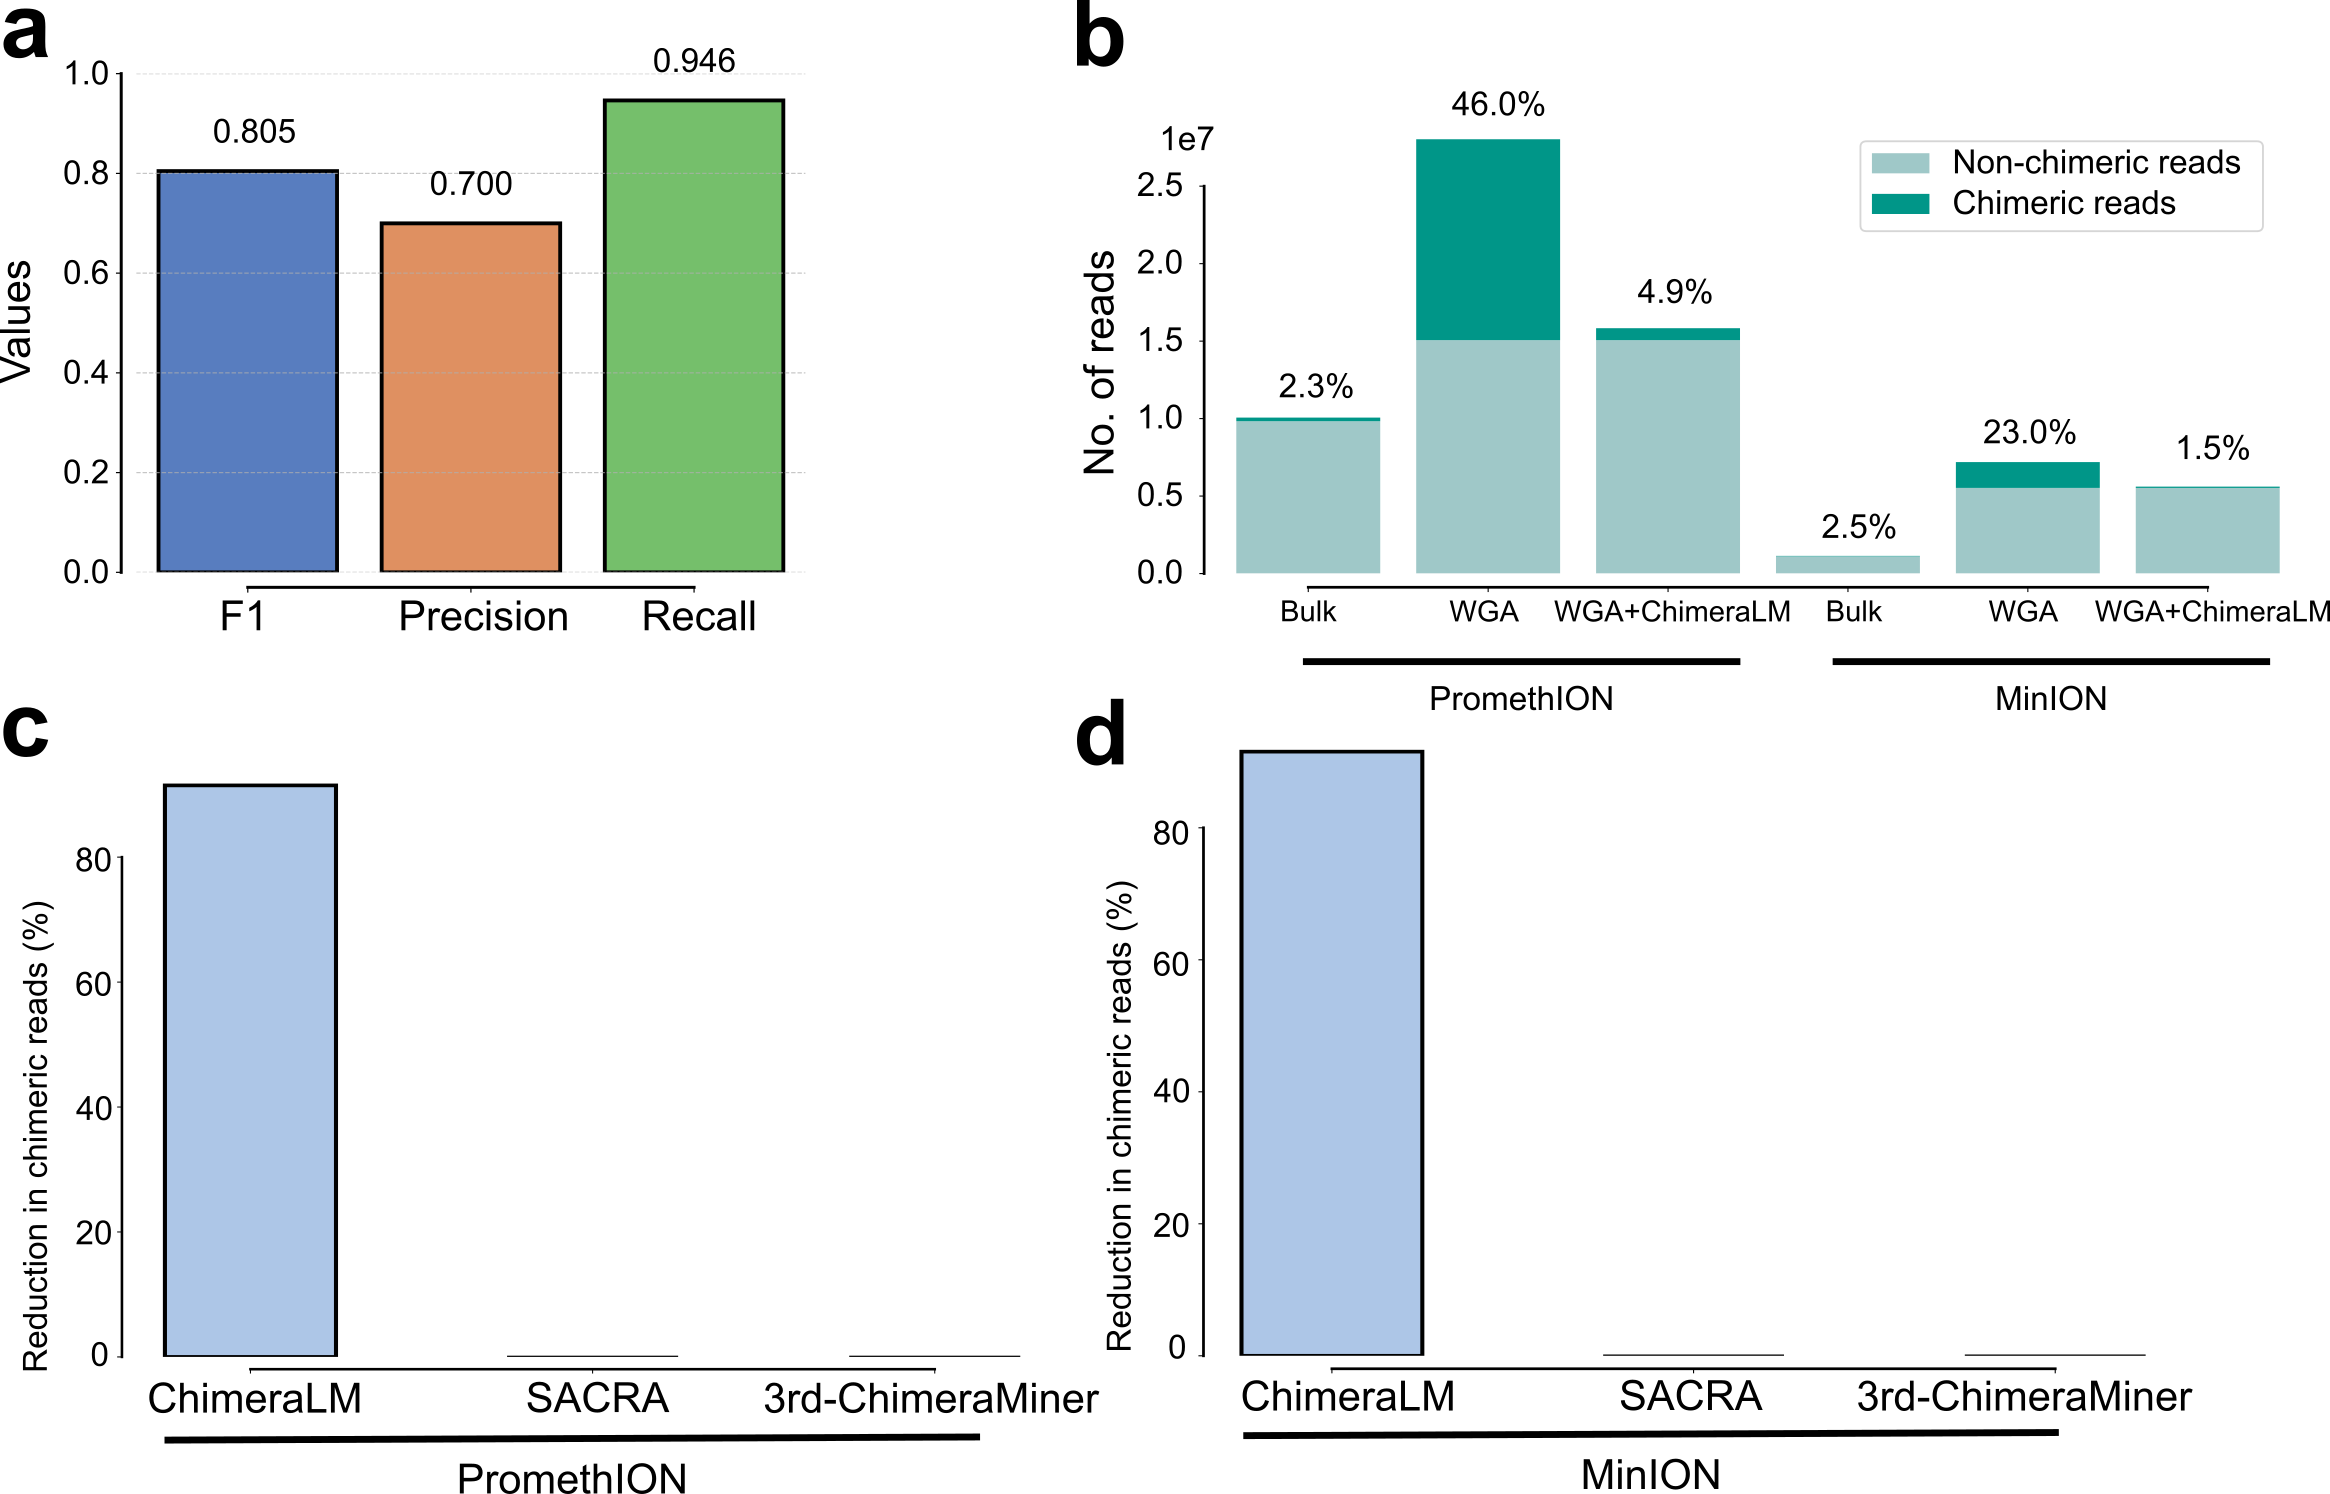
\includegraphics[width=0.95\textwidth]{final_figures/figure2}
	\end{center}
    \caption{{\bf ChimeraLM accurately identifies and removes \gls{wga}-induced chimeric artifacts.}
	(a)~Classification performance on held-out test data.
    ChimeraLM achieves high recall (0.95) in identifying chimeric reads while maintaining acceptable precision (0.70), yielding an F1 score of 0.81 for binary classification of biological versus artifactual sequences.
	(b)~Chimeric read reduction across sequencing platforms.
    Stacked bars show the proportion of chimeric (dark teal) and non-chimeric (light teal) reads in bulk sequencing, \gls{wga}-amplified samples, and ChimeraLM-filtered \gls{wga} samples.
    Data from PC3 cell line sequenced on PromethION (left) and MinION (right) platforms demonstrate that ChimeraLM reduces chimeric read frequencies from 46.0\% to 4.9\% (PromethION) and from 23.0\% to 1.5\% (MinION), approaching bulk levels (2.3\% and 2.5\%, respectively).
	(c,d)~Benchmarking against existing methods.
    ChimeraLM achieves approximately 90\% reduction in chimeric reads on both PromethION (c) and MinION (d) platforms, whereas existing computational tools SACRA and 3rd-ChimeraMiner show no detectable reduction in chimeric content.}\label{fig:figure2}
\end{figure}

\subsection*{ChimeraLM accurately distinguishes biological reads from chimeric artifacts}
We evaluated ChimeraLM's classification accuracy on held-out test data comprising reads with known biological or chimeric status (Fig.~\ref{fig:figure2}a).
The model achieved an F1 score of 0.81, balancing the competing demands of sensitivity and specificity in artifact detection. 

ChimeraLM demonstrated high recall (0.95), successfully identifying 95\% of true chimeric artifacts in the test dataset.
This high sensitivity is critical for single-cell genomic analyses, as it ensures that most amplification-induced artifacts are removed before structural variant calling, preventing false-positive variant detection.
The model's precision of 0.70 indicates that 70\% of reads flagged as chimeric were true artifacts, while 30\% were biological reads incorrectly classified as artificial.

This precision-recall trade-off reflects a deliberate design choice that prioritizes comprehensive artifact removal over perfect specificity.
Retaining chimeric reads leads to false \gls{sv} calls that can misrepresent cellular genotypes, whereas removing some biological reads reduces sequencing depth but does not introduce false biological conclusions.
For typical single-cell \gls{wga} samples with 20-30× coverage, the loss of 30\% of reads in chimera-dense regions still maintains sufficient depth (14-21×) for reliable variant calling, while the removal of 95\% of chimeric artifacts substantially improves variant detection accuracy.
This balance makes ChimeraLM practical for single-cell genomic studies where eliminating technical artifacts is paramount to identifying genuine biological variation.

\subsection*{ChimeraLM reduces chimeric artifacts to near-bulk levels across sequencing platforms}
To assess ChimeraLM's practical effectiveness, we applied the trained model to PC3 cell line \gls{wga} data sequenced on two Nanopore platforms: PromethION and MinION (Fig.~\ref{fig:figure2}b). 
ChimeraLM was trained using a subset of PromethION data, where chimeric artifacts were identified by comparison with bulk sequencing, then subsampled to create balanced training examples~\ref{subsec:train_data}. 
Importantly, not all chimeric reads from PromethION were used during training, allowing evaluation on both seen and unseen examples.

Bulk sequencing without amplification established baseline chimeric rates of 2.3\% (PromethION) and 2.5\% (MinION), representing the low background level of sequencing artifacts in non-amplified samples. 
\gls{wga} dramatically increased chimeric contamination to 46.0\% on PromethION and 23.0\% on MinION, confirming that \gls{wga} introduces substantial artifactual content.

When applied to the full PromethION dataset (including chimeric reads not seen during training), ChimeraLM reduced chimeric content from 46.0\% to 4.9\%, retaining 15.8 million biological reads from 28.0 million total reads.
On the independent MinION platform, ChimeraLM reduced chimeric reads from 23.0\% to 1.5\%, approaching bulk sequencing quality (2.5\%) while preserving 5.6 million reads from 7.2 million total.
This represents approximately a 10-fold (PromethION) and 15-fold (MinION) reduction in chimeric artifacts.

The strong performance on both unseen PromethION reads and the independent MinION platform demonstrates that ChimeraLM learns generalizable sequence features distinguishing biological reads from chimeric artifacts, rather than memorizing training examples or platform-specific signatures.
This generalization is critical for practical application, enabling users to apply ChimeraLM across different datasets and sequencing platforms without retraining.

\subsection*{Existing chimera detection tools do not effectively process nanopore sequencing data}
% P2 92 
% mk1c 91
We compared ChimeraLM's performance to existing computational methods for detecting amplification-induced chimeric sequences: SACRA~\cite{kiguchi2021longread} and 3rd-ChimeraMiner~\cite{lu2023exploration} (Fig.~\ref{fig:figure2}c,d). 
SACRA was developed for detecting chimeras in \gls{wga} coupled with \gls{pb} long-read sequencing, specifically for metagenomic applications.
3rd-ChimeraMiner was also designed for MDA-amplified samples sequenced on the \gls{pb} platform, focusing on recognizing and restoring chimeric structures to their original genomic configurations.

We applied both tools to our PC3 \gls{wga} data sequenced on nanopore platforms (PromethION and MinION).
Neither SACRA nor 3rd-ChimeraMiner achieved a detectable reduction in chimeric reads on either platform, showing 0\% reduction compared to unprocessed data, while ChimeraLM reduced chimeric content by approximately 90\% on both platforms (Fig.~\ref{fig:figure2}c,d).
It is important to note that we tested these tools outside their intended platform context—both were designed and validated for \gls{pb} sequencing, not \gls{ont}.
The failure of these tools on nanopore data likely reflects fundamental platform incompatibilities rather than limitations in their original design.

ChimeraLM addresses the need for nanopore-specific chimera detection through a sequence-only deep learning approach.
By training directly on nanopore \gls{wga} data, the model learns sequence-level patterns that distinguish biological reads from chimeric artifacts as they appear in nanopore sequencing. This platform-specific training is essential for effective chimera detection, as demonstrated by the performance differences observed.
Our results highlight that nanopore-based single-cell genomics requires dedicated bioinformatics tools optimized for the platform's unique characteristics, rather than adaptation of methods from other sequencing technologies.

\begin{figure}[H]
	\begin{center}
		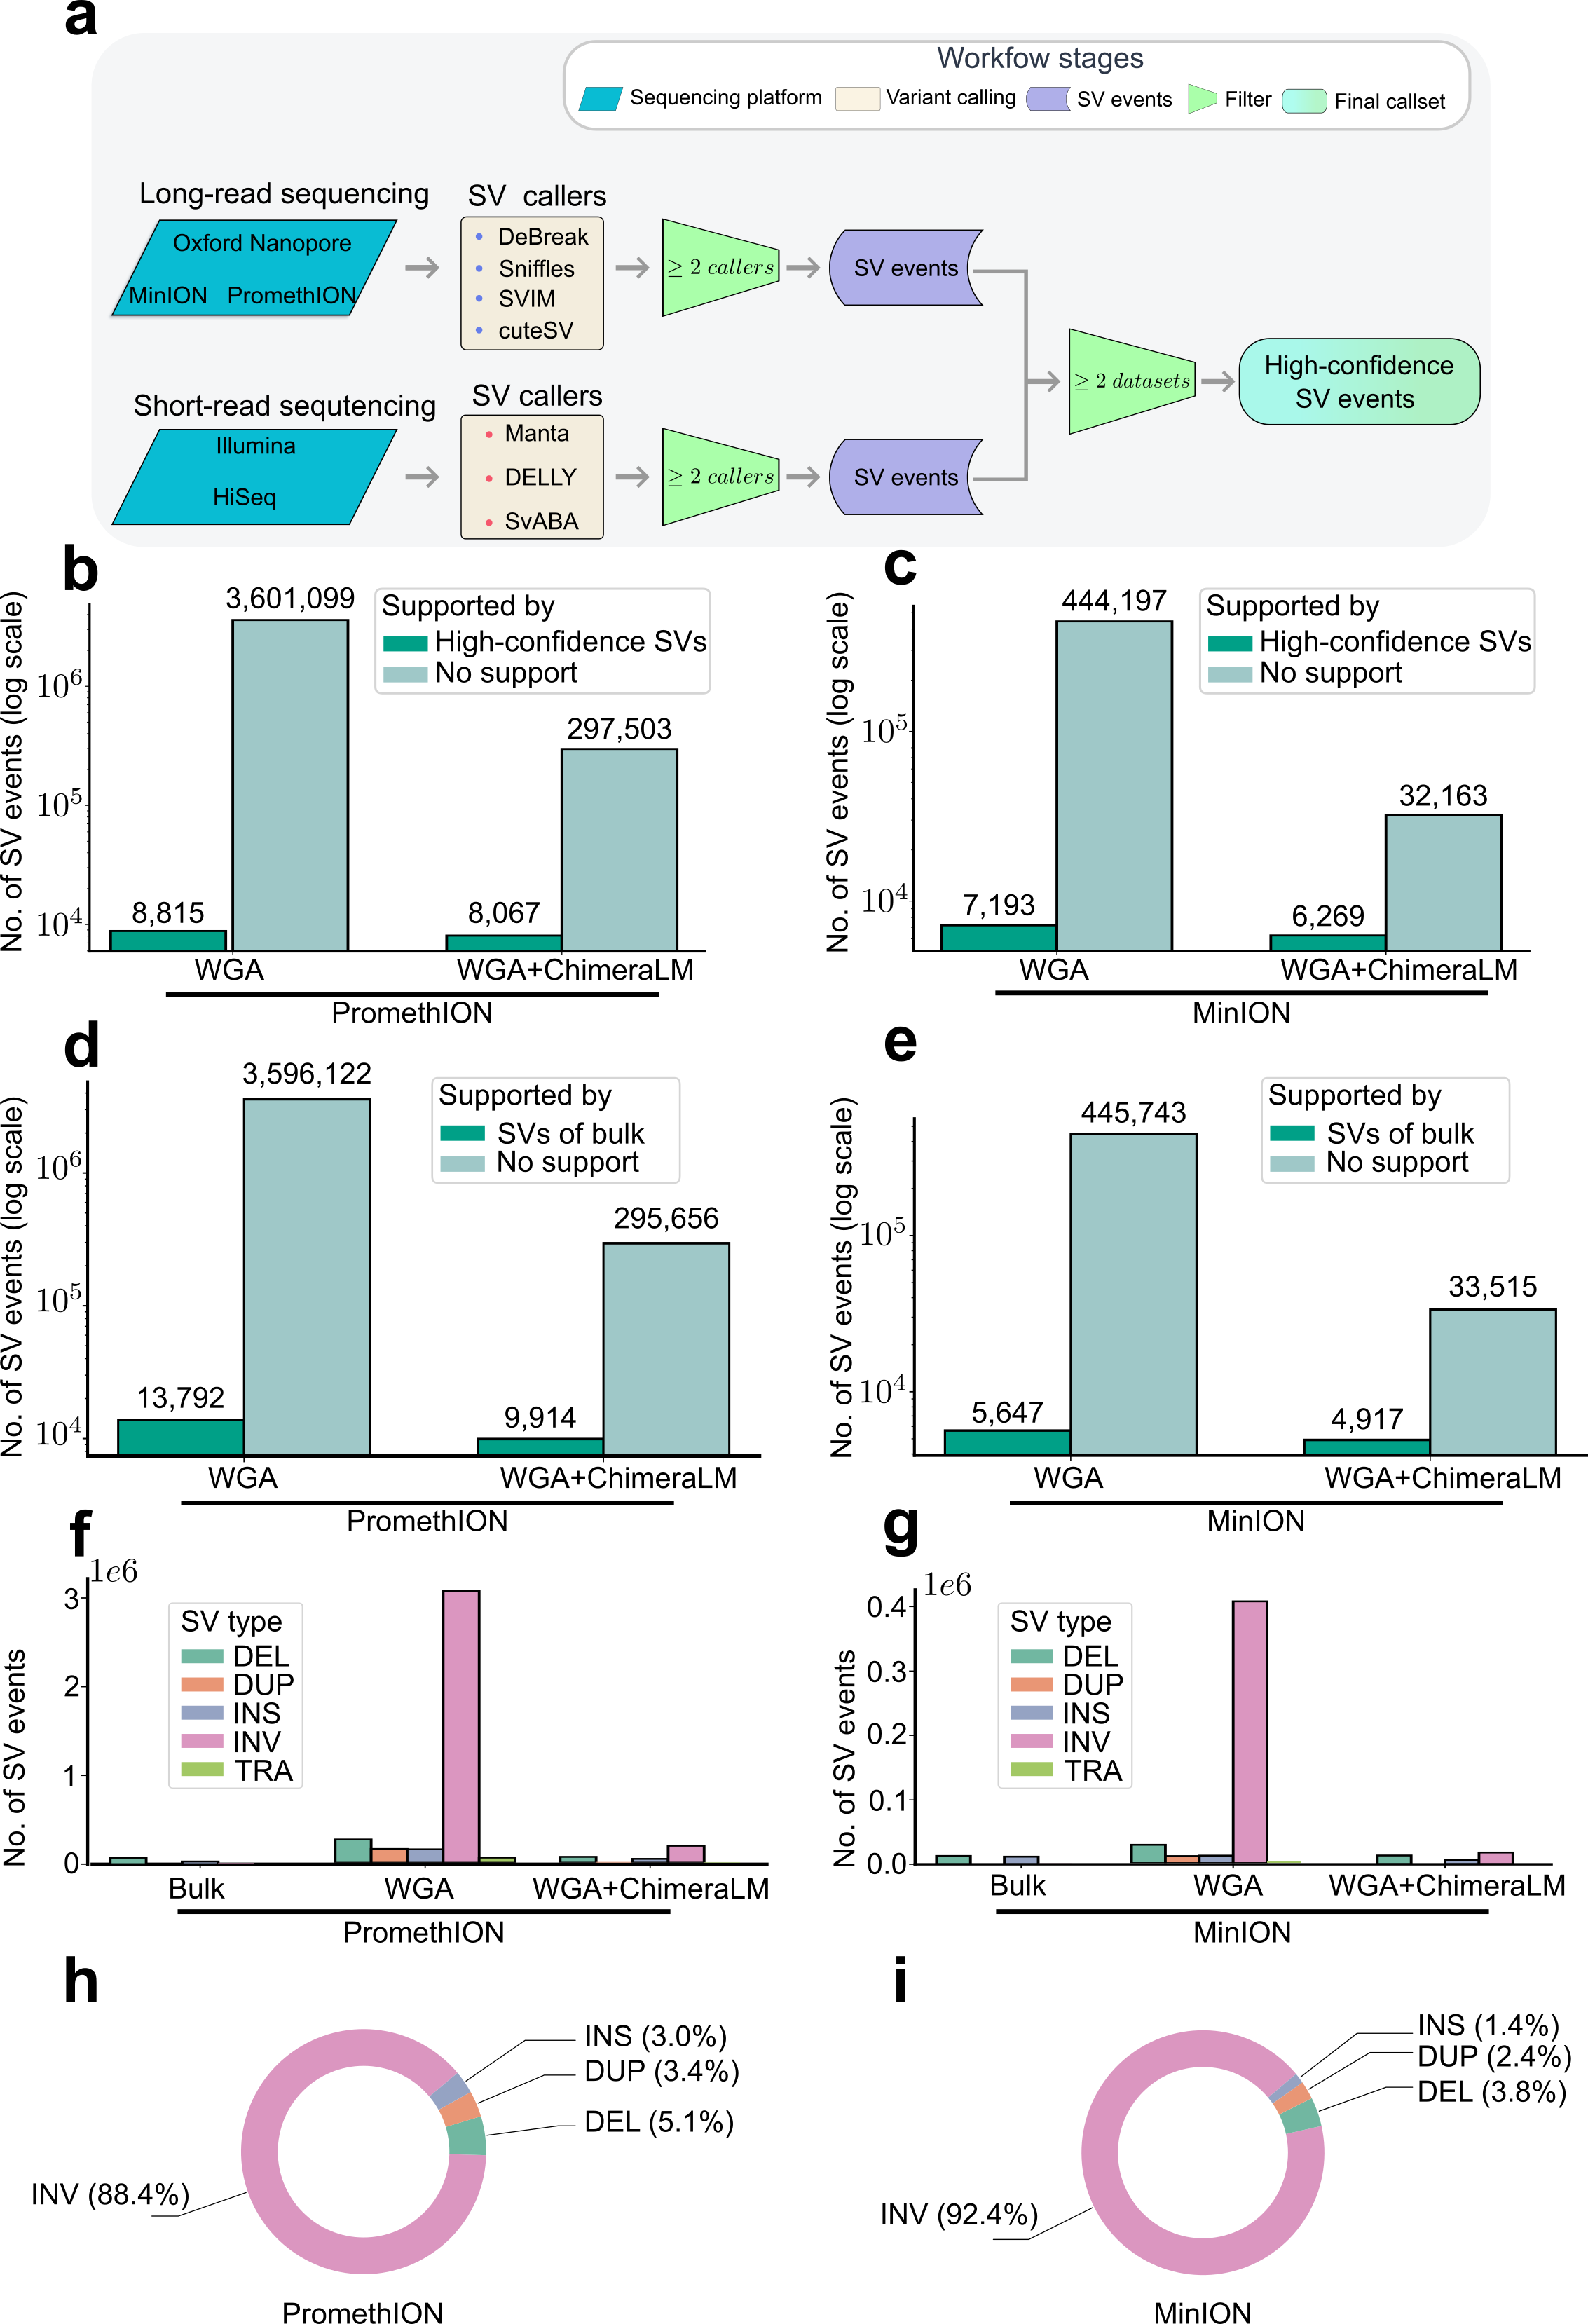
\includegraphics[width=0.95\textwidth]{final_figures/figure3}
	\end{center}
	\caption{{\bf ChimeraLM filtering improves structural variant detection accuracy.}
		(a)~Construction of high-confidence \gls{sv} reference dataset. PC3 bulk DNA was sequenced on multiple platforms (\gls{ont} PromethION and MinION, Illumina HiSeq) and analyzed with multiple \gls{sv} calling algorithms. \gls{sv} events detected by $\geq$2 callers on the same platform were retained. Events supported by both long-read and short-read platforms were designated as high-confidence gold standard \glspl{sv}.
		(b,c)~\gls{sv} validation against multi-platform gold standard. Stacked bars show total \gls{sv} calls (log scale, numbers above bars) classified as gold standard-supported (dark teal) or unsupported (light teal) for PromethION (b) and MinION (c). ChimeraLM filtering substantially reduces unsupported \gls{sv} calls while preserving gold standard events.
		(d,e)~\gls{sv} validation against long-read bulk sequencing (\gls{ont} PromethION and MinION). Stacked bars show \gls{sv} calls classified as bulk-supported (dark teal) or bulk-unsupported (light teal) for PromethION (d) and MinION (e). Long-read bulk data from the same platform provides platform-matched validation, capturing true variants that may be specific to long-read detection.
		(f,g)~\gls{sv} type distribution across processing methods. Bar charts show the number of detected \glspl{sv} by type: \gls{del} (green), \gls{dup} (orange), \gls{ins} (blue), \gls{inv} (pink), and \gls{tra} (light green) for PromethION (f) and MinION (g). Unfiltered \gls{wga} data shows elevated counts across all types, particularly inversions and translocations, which are reduced to bulk-like levels after ChimeraLM filtering.
		(h,i)~Composition of chimeric artifact-supported \glspl{sv}. Pie charts show the proportion of \gls{sv} types among events supported exclusively by reads classified as chimeric artifacts in unfiltered \gls{wga} data for PromethION (h) and MinION (i). These represent false-positive \gls{sv} calls that would be eliminated by ChimeraLM filtering.
	}\label{fig:figure3}
\end{figure}


\subsection*{ChimeraLM substantially reduces false-positive structural variant calls}

Accurate \gls{sv} detection is essential for understanding genomic diversity and disease mechanisms in single cells.
However, \gls{wga}-induced chimeric artifacts can be misidentified as genuine \glspl{sv}, leading to incorrect biological conclusions.
To quantify ChimeraLM's impact on downstream \gls{sv} detection accuracy, we compared variant calls from unfiltered \gls{wga} data versus ChimeraLM-filtered data against two independent reference standards.

We first constructed a high-confidence gold standard \gls{sv} dataset by integrating multiple sequencing platforms and detection algorithms (Fig.~\ref{fig:figure3}a).
PC3 bulk DNA was sequenced using long-read (\gls{ont} PromethION and MinION) and short-read (Illumina HiSeq) technologies (Extended Table~\ref{tab:seq_stats}).
\glspl{sv} detected by $\geq$2 calling algorithms on the same platform and supported by both long-read and short-read data were designated as gold standard events.
This multi-platform consensus approach ensures high specificity, as true \glspl{sv} should be detectable across different sequencing technologies.

When comparing \gls{wga} samples against the gold standard, unfiltered data showed extensive false-positive \gls{sv} calls (Fig.~\ref{fig:figure3}b,c).
On PromethION, raw \gls{wga} data produced 3.6 million \gls{sv} calls, of which only 8,815 (0.24\%) matched gold standard events—meaning 99.76\% of calls were likely artifacts.
ChimeraLM filtering reduced total calls to 305,570 while retaining 8,067 gold standard events, increasing the validation rate to 2.64\% (11-fold improvement) and preserving 91.5\% of true variants.
MinION data showed similar results: \gls{wga} produced 451,390 calls with 1.59\% validation rate, while ChimeraLM-filtered data yielded 38,432 calls with a 16.3\% validation rate (10-fold improvement) and 87.2\% true variant retention.

To complement the stringent gold standard validation, we also compared \gls{sv} calls against long-read bulk sequencing from the same platform (Fig.~\ref{fig:figure3}d,e).
This platform-matched validation captures true \glspl{sv} that may be detectable specifically in long-read data but missed by short-read sequencing, providing a more inclusive reference for evaluating recall.
On PromethION bulk validation, ChimeraLM filtering increased the validation rate from 0.38\% to 3.24\% (8.5-fold improvement) while retaining 71.9\% of bulk-supported events.
MinION bulk validation showed similar improvements, with validation rates increasing from 1.25\% to 12.79\% (10-fold improvement) and 87.1\% retention of bulk-supported events.

These results have important practical implications.
The 8-16 fold reduction in false-positive rate means researchers can focus on biologically relevant \glspl{sv} without manually filtering thousands of artificial calls.
The high retention of true variants (72-92\% depending on validation stringency) ensures that ChimeraLM filtering does not compromise detection sensitivity for genuine genomic alterations. Together, these metrics demonstrate that ChimeraLM substantially improves the signal-to-noise ratio in single-cell \gls{sv} detection, making downstream biological interpretation more reliable and efficient.

\subsection*{ChimeraLM restores structural variant type distributions to bulk sequencing profiles}

We compared the distribution of \gls{sv} types across bulk, unfiltered \gls{wga}, and ChimeraLM-filtered samples to assess whether artifact removal normalizes \gls{sv} profiles (Fig.~\ref{fig:figure3}f,g).
Bulk sequencing exhibited relatively balanced distributions across \glspl{del}, \glspl{dup}, \glspl{ins}, \glspl{inv}, and \glspl{tra}.
In contrast, unfiltered \gls{wga} data showed dramatically skewed distributions dominated by \glspl{inv} on both PromethION and MinION platforms.
This disproportionate \gls{inv} enrichment is consistent with their artificial origin: chimeric reads created by template switching during \gls{wga} produce alignment patterns that mimic genuine \glspl{inv}~\cite{lu2023chimera, agyabeng2025evaluating}.

ChimeraLM filtering substantially normalized these distributions toward bulk profiles.
The overwhelming excess of \glspl{inv} was dramatically reduced on both platforms, while other \gls{sv} types were maintained at levels consistent with bulk sequencing.
This normalization occurred through selective removal of artifact-supported \glspl{inv} rather than indiscriminate elimination of all \gls{inv} calls.
The restoration of biologically representative \gls{sv} type distributions enables accurate characterization of \gls{sv} in single cells without the confounding effects of amplification artifacts.

\subsection*{Deep learning classification reveals chimeric artifact-associated structural variants}

ChimeraLM's read-level classification enables a new type of analysis: identifying which \gls{sv} calls are associated with chimeric versus biological reads (Fig.~\ref{fig:figure3}h,i).
Analysis of \glspl{sv} supported exclusively by ChimeraLM-identified chimeric artifacts showed that \glspl{inv} strongly dominate (88.4\% on PromethION, 92.4\% on MinION), consistent with how chimeric junctions create alignment signatures resembling genuine inversions~\cite{lu2023chimera, agyabeng2025evaluating}.
The remaining calls included \glspl{del} (5.1\% PromethION, 3.8\% MinION), \glspl{dup} (3.4\%, 2.4\%), and \glspl{ins} (3.0\%, 1.4\%).
For these other SV types, interpretation is less certain—some may represent genuine \glspl{sv} that happen to be supported by chimeric reads locally, while others may be artifacts from specific junction configurations.

These results demonstrate that without ChimeraLM, genomic studies would be severely compromised by false-positive \gls{inv} calls, potentially leading to misinterpretation of chromosomal instability, copy number profiles, and other key genomic features~\cite{kosugi2019comprehensive, mahmoud2019structural}.
ChimeraLM's ability to identify and remove these specific artifacts represents a critical advancement for accurate \gls{sv} analysis.

\begin{figure}[H]
	\begin{center}
		\includegraphics[width=\textwidth]{final_figures/figure4}
	\end{center}
	\caption{{\bf ChimeraLM attention weights localize to chimeric junction regions.}
		(a,d)~Attention weight profiles for two representative chimeric reads. Upper panels show attention weights per sequence position (blue line) and mean attention (dashed line). Red vertical lines mark chimeric junction positions, with pink shading indicating junction windows ($\pm$50~bp). Purple arrows show reported \gls{sv} breakpoints. Lower panels illustrate read alignments: reads (top bars) show orientation transitions at junctions (green = forward, red = reverse-complemented, arrows indicate strand), while reference genome (bottom bars) maintains continuous forward orientation. Gray regions connect aligned segments.
		(b,e)~Quantitative attention analysis. Box plots show significantly elevated attention weights in junction region versus non-junction regions for both examples ($p = 5.3 \times 10^{-14}$ and $p = 6.8 \times 10^{-15}$, respectively; Wilcoxon rank-sum test).
		(c,f)~Proposed chimera formation mechanisms. Step 1: Original DNA fragments from distant genomic loci exist in forward orientation. Step 2: During \gls{wga}, one or both fragments may undergo random reverse-complementation. Step 3: Template switching joins the fragments with discordant orientations, creating chimeric artifacts. The two examples illustrate different orientation patterns (forward-to-reverse vs reverse-to-forward transitions) arising from random strand selection during amplification.
	}\label{fig:figure4}
\end{figure}

\subsection*{ChimeraLM demonstrates capacity to learn biologically relevant sequence features}

To understand which sequence features ChimeraLM uses for classification, we examined the attention weights from the model's pooling mechanism.
Attention weights indicate which nucleotide positions most strongly influence classification decisions, providing potential interpretability into the model's learned patterns.

We identified cases where ChimeraLM assigns elevated attention weights to chimeric junction regions—the breakpoints where template switching artificially joins DNA fragments from different genomic loci (Fig.~\ref{fig:figure4}a,d).
In these representative examples, attention profiles show predominantly low baseline weights across most of the read length, with pronounced peaks at junction sites where sequence orientation transitions occur.
At these junctions, reads exhibit characteristic discordant alignment patterns: one segment aligns in reverse orientation while the adjacent segment aligns forward to a distant genomic location, creating the structural signature of \gls{wga}-induced chimeric artifacts.

Quantitative analysis of these examples confirmed that attention weights within junction regions ($\pm$50~bp) were significantly elevated compared to background regions ($p = 5.3 \times 10^{-14}$ and $p = 6.8 \times 10^{-15}$, Wilcoxon rank-sum test) (Fig.~\ref{fig:figure4}b,e).
The localization pattern in these cases suggests ChimeraLM can learn mechanistically relevant features: the orientation discontinuities created when DNA fragments are artificially joined during amplification (Fig.~\ref{fig:figure4}c,f).

However, we note that not all chimeric reads exhibit such clearly interpretable attention patterns.
Some chimeric reads show more diffuse attention distributions without obvious localization to junctions, suggesting that ChimeraLM may use multiple complementary features for classification—including junction signatures when present, but also other sequence characteristics such as compositional biases, k-mer patterns, or context-dependent features.
This heterogeneity in attention patterns likely reflects the diverse nature of chimeric artifacts, which can vary in junction structure, fragment length, and local sequence context.

Despite this variability, the existence of interpretable cases provides valuable insights.
It demonstrates that ChimeraLM has the capacity to learn biologically meaningful structural features when junction signatures are prominent, validating that the model captures aspects of the underlying chimera formation mechanism.
The attention weights also provide a useful tool for inspecting individual predictions, particularly for high-confidence classifications where junction localization may aid manual review.

\section*{Discussion}\label{sec:discussion}

\gls{wga} has enabled genomic analysis from single cells but introduces chimeric artifacts that compromise \gls{sv} detection.
ChimeraLM addresses this challenge through sequence-level classification of biological versus artificial reads, substantially improving \gls{sv} calling accuracy before downstream analysis.
This upstream filtering approach—removing problematic sequences at the read level rather than attempting to correct errors after variant calling—provides a practical solution for single-cell genomics laboratories.

Our results demonstrate several key advantages of ChimeraLM over existing approaches.
First, the method achieves approximately 90\% reduction in chimeric reads across different nanopore sequencing platforms while retaining 87-92\% of true \glspl{sv}.
Second, ChimeraLM reduces false-positive \gls{sv} calls by 8-16 fold, enabling researchers to focus on biologically relevant variants without manual filtering of thousands of artificial calls.
Third, the approach works across PromethION and MinION platforms without platform-specific retraining, indicating that the model learns generalizable sequence features of \gls{wga}-induced chimeras.

ChimeraLM's effectiveness reflects the ability of deep learning models to capture complex sequence patterns that are difficult to encode in rule-based filters.
Traditional quality control approaches rely on predefined criteria such as mapping quality or read depth~\cite{kiguchi2021longread, lu2023exploration}, which may not effectively distinguish chimeric artifacts from biological sequences.
By learning directly from data, ChimeraLM discovers subtle compositional and structural features that distinguish authentic genomic sequences from amplification artifacts.
The attention weight analysis provides evidence that the model can identify mechanistically relevant features such as orientation discontinuities at chimeric junctions, though the heterogeneity in attention patterns across reads suggests the model uses multiple complementary features for classification.

The improved reliability of \gls{sv} detection has practical implications for single-cell genomics applications.
Studies of chromosomal instability, clonal evolution, and \gls{sv} burden in individual cells have been limited by high false-positive rates in \gls{wga} data~\cite{kosugi2019comprehensive, mahmoud2019structural}.
ChimeraLM enables more confident identification of genuine \glspl{sv}, supporting applications in cancer genomics, developmental biology, and aging research where single-cell resolution is essential for understanding cellular heterogeneity.

Several limitations warrant consideration.
ChimeraLM was trained and validated on PC3 cell line data using \gls{mda}-based \gls{wga} and nanopore sequencing.
Performance on other cell types, \gls{wga} chemistries (PicoPLEX, LIANTI), or sequencing platforms (\gls{pb}) remains to be systematically evaluated.
Amplification biases may vary across genomic backgrounds with different chromatin states or DNA accessibility, potentially affecting model generalization.

% The binary classification approach assumes a clear distinction between biological and artifactual sequences.
% However, some complex structural rearrangements can produce reads resembling chimeric artifacts.
% ChimeraLM may incorrectly classify such genuine but complex rearrangements as artifacts, potentially leading to loss of biologically important events.
% Future developments could incorporate multi-class classification or confidence scoring to handle ambiguous cases.

Future work should prioritize validation across diverse biological contexts.
Testing on multiple cell types (primary cells, stem cells, immune cells) and \gls{wga} protocols will establish generalizability.
Evaluation on \gls{pb} long-read data would determine whether the approach extends to circular consensus sequencing.
% Integration with additional sequencing modalities (linked-reads, strand-seq) could provide complementary information for chimera detection.

% The interpretability of attention-based models could be leveraged to provide insights into \gls{wga} artifact formation mechanisms.
% Systematic analysis of attention patterns across thousands of chimeric reads may reveal common sequence motifs, structural features, or genomic contexts associated with template switching. Such insights could inform development of improved amplification protocols or guide targeted optimization of \gls{wga} chemistry.

More broadly, ChimeraLM demonstrates the utility of genomic language models for quality control applications~\cite{nguyen2023hyenadna}.
Similar deep learning approaches could address other data quality challenges in genomics, including contamination detection, adapter artifact identification, or systematic error correction in diverse sequencing technologies.
As foundation models for biological sequences continue to advance, quality control and data preprocessing may emerge as important application domains alongside traditional prediction tasks.

ChimeraLM provides a practical and effective tool for improving single-cell genomic data quality. By removing \gls{wga}-induced chimeric artifacts at the read level, the method enables more reliable \gls{sv} detection and supports biological applications that require accurate characterization of genomic variation at single-cell resolution.


% ChimeraLM demonstrates that sophisticated computational approaches can effectively address fundamental technical challenges that have limited single-cell genomics.
% By providing a robust solution to chimeric artifact detection, this work removes a significant barrier to reliable single-cell genomic analysis and opens new possibilities for biological discovery and clinical application.
% As single-cell approaches become increasingly central to modern biology and medicine, computational tools like ChimeraLM will be essential for realizing their full potential.


\section*{Methods}\label{sec:methods}

\subsection*{Cell culture, single-clone preparation, and nanopore sequencing}

\paragraph{Cell culture and single-clone establishment}
PC3 prostate cancer cells (ATCC\textsuperscript{\textregistered} CRL-1435\texttrademark) were cultured in RPMI-1640 medium supplemented with 10\% fetal bovine serum and 1\% penicillin--streptomycin at 37~\textdegree C with 5\% CO\textsubscript{2}. To minimize biological heterogeneity, a monoclonal population was established by serial dilution in 96-well plates, ensuring that each culture originated from a single cell. Mycoplasma contamination was routinely tested and confirmed negative prior to DNA extraction.

\paragraph{DNA extraction and whole-genome amplification}
From the monoclonal population, two types of DNA samples were prepared: a bulk (non-amplified) control and ten single-cell MDA-amplified genomes. Bulk high-molecular-weight DNA was extracted using the Monarch\textsuperscript{\textregistered} HMW DNA Extraction Kit for Cells \& Blood (New England Biolabs). Individual cells were isolated using 1CellDish-60~mm (iBiochips) and amplified using the REPLI-g Advanced DNA Single Cell Kit (Qiagen) following the manufacturer's protocol. DNA concentration and fragment integrity were assessed with a Qubit~4 fluorometer and Agilent TapeStation (DNA~1000/5000 ScreenTape). Only samples meeting quality standards were used for library construction.

\paragraph{Nanopore library preparation and sequencing}
Sequencing libraries were prepared using the \gls{ont} Ligation Sequencing Kit~V14 (SQK-LSK114) and sequenced on MinION~Mk1C or PromethION~P2~Solo devices with R10.4.1 flow cells according to the manufacturer's genomic DNA workflow. Because all single-cell samples originated from the same monoclonal lineage, observed differences between amplified and bulk data primarily reflect MDA-induced artifacts rather than biological variation, providing a controlled experimental setting for downstream analyses.

\paragraph{Basecalling and read processing}
Raw signal files (POD5) were basecalled using Dorado~v0.5.0 with the high-accuracy model \texttt{dna\_r10.4.1\_e8.2\_400bps\_hac@v4.3.0}~\cite{dorado2023}. Reads with mean quality $< 10$ or length $< 500$~bp were removed. Residual adapters and concatemers were trimmed using Cutadapt~v4.0~\cite{martin2011cutadapt} in two-pass error-tolerant mode. Cleaned reads were aligned to the GRCh38.p13 reference genome using minimap2~v2.26 (\texttt{map-ont} preset)~\cite{li2018minimap2}. Resulting BAM files were sorted and indexed with SAMtools~v1.16~\cite{danecek2021twelve}. All samples were processed under identical parameters to ensure consistency across datasets.

\paragraph{Chimeric read identification}
Chimeric reads were identified based on the presence of supplementary alignments in BAM files using the \gls{sa} tag.
The \gls{sa} tag indicates that a read has additional alignments beyond the primary alignment, which is characteristic of chimeric sequences that map to multiple distant genomic locations.
To ensure accurate identification, we applied stringent filtering criteria: reads were classified as chimeric only if they (1) contained the \gls{sa} tag, (2) were not unmapped, (3) were not secondary alignments, and (4) were not supplementary alignments themselves.
This filtering approach ensures that only primary alignments with supplementary mapping evidence are considered chimeric, avoiding double-counting of the same chimeric event and excluding low-quality or ambiguous alignments.
Reads without the \gls{sa} tag (single continuous alignments) were classified as non-chimeric.
This approach leverages the standard BAM format specification to reliably identify reads with complex alignment patterns.

\subsection*{Training data construction}

\paragraph{Training data generation}
We generated training data from PC3 cells using \gls{wga} sequencing on the PromethION P2 platform (\gls{ont}) and three independent bulk sequencing datasets: bulk sequenced on PromethION P2, bulk sequenced on MinION Mk1c (\gls{ont}), and bulk sequenced on PacBio.
\gls{wga} data sequenced on MinION Mk1c was reserved as a completely independent test set.
Bulk sequencing from non-amplified genomic DNA serves as reference data containing only genuine biological sequences, while \gls{wga} sequencing from amplified DNA contains both authentic genomic sequences and amplification-induced chimeric artifacts.

\paragraph{Ground truth labeling}
We first labeled chimeric reads from \gls{wga} PromethION P2 data by comparing them against chimeric reads from all three bulk datasets.
For each \gls{wga} chimeric read, we extracted all alignment segments (defined by start-end positions on the reference genome) and compared them against alignment segments from bulk chimeric reads.
A \gls{wga} read was labeled as biological if all its alignment segments matched corresponding segments from at least one bulk chimeric read within a 1~kb position threshold, indicating the chimeric structure exists in non-amplified DNA.
\gls{wga} reads whose alignment segment patterns did not match any bulk chimeric reads across all three datasets were labeled as artificial chimeras generated during amplification.
To augment the biological class, we subsampled chimeric reads from all three bulk datasets and labeled them as biological, as chimeric reads in non-amplified bulk DNA represent genuine biological events (e.g., true \glspl{sv}).
The final training dataset combined the labeled \gls{wga} PromethION P2 reads with the subsampled bulk chimeric reads.

\paragraph{Dataset partitioning and cross-platform validation}
The combined labeled dataset was partitioned into training (70\%), validation (20\%), and test (10\%) sets using stratified random sampling.
The training set was used for model parameter optimization, the validation set for hyperparameter tuning and monitoring training progress, and the test set for final performance evaluation.
The \gls{wga} MinION Mk1c dataset served as a completely independent test set for evaluating cross-platform generalization, as it was sequenced on a different nanopore platform and never exposed to the model during development.
This design tests whether ChimeraLM learns generalizable sequence features of \gls{wga}-induced chimeric artifacts rather than platform-specific technical signatures.

\subsection*{Model architecture}

\paragraph{Backbone encoder}
ChimeraLM employs the pre-trained HyenaDNA model~\cite{nguyen2023hyenadna} as its backbone encoder.
This model was pre-trained on large-scale genomic data and provides robust sequence representations.
DNA sequences are tokenized at single-nucleotide resolution, with each base (A, C, G, T, N) mapped to a unique integer token (7, 8, 9, 10, 11, respectively).
Special tokens include [CLS]=0, [PAD]=4, and others for sequence processing.
Input sequences are truncated at 32,768 bp or padded to enable batch processing.

For a tokenized input sequence $\mathbf{x} \in \mathbb{Z}^{L}$, the HyenaDNA backbone generates contextualized hidden representations:
$$
\mathbf{H} = \text{HyenaDNA}(\mathbf{x}) \in \mathbb{R}^{L \times 256}
$$
where $\mathbf{H} = (\mathbf{h}_1, \mathbf{h}_2, \ldots, \mathbf{h}_L)$ represents position-wise hidden states with dimension 256. 
The Hyena operators~\cite{Poli2023HyenaHT} efficiently capture both local sequence motifs and long-range dependencies essential for distinguishing biological sequences from chimeric artifacts.

\paragraph{Attention pooling}
To aggregate variable-length sequence representations into fixed-size vectors, ChimeraLM implements attention-based pooling. 
For hidden states $\mathbf{H} \in \mathbb{R}^{L \times 256}$, attention weights are computed through a two-layer network:
\begin{align*}
\mathbf{e} &= \text{GELU}(\text{Linear}_{256 \to 256}(\mathbf{H})) \in \mathbb{R}^{L \times 256} \\
\mathbf{s} &= \text{Linear}_{256 \to 1}(\mathbf{e}) \in \mathbb{R}^{L \times 1} \\
\boldsymbol{\alpha} &= \text{softmax}(\mathbf{s}) \in \mathbb{R}^{L \times 1}
\end{align*}
The pooled representation is the weighted sum of hidden states:
$$
\mathbf{h}_{\text{pooled}} = \sum_{i=1}^{L} \alpha_i \mathbf{h}_i \in \mathbb{R}^{256}
$$
This mechanism assigns learned importance weights to each sequence position, enabling the model to focus on informative regions while accommodating natural variability in read lengths.

\paragraph{Classification head}
The pooled representation is processed through a \gls{mlp} with residual connections.
The first layer expands dimensionality:
$$
\mathbf{f}_1 = \text{Dropout}_{0.1}(\text{GELU}(\text{Linear}_{256 \to 512}(\mathbf{h}_{\text{pooled}}))) \in \mathbb{R}^{512}
$$
Subsequent residual blocks with input $\mathbf{f}_{\text{in}} \in \mathbb{R}^{512}$ compute:
$$
\mathbf{f}_{\text{out}} = \text{Dropout}_{0.1}(\text{Linear}_{512 \to 512}(\text{GELU}(\text{Linear}_{512 \to 512}(\mathbf{f}_{\text{in}}))))) + \mathbf{f}_{\text{in}}
$$
where the skip connection enables stable gradient flow during training.
The final layer produces binary classification logits:
$$
\mathbf{z} = [z_0, z_1] = \text{Linear}_{512 \to 2}(\mathbf{f}_{\text{final}}) \in \mathbb{R}^{2}
$$
where $z_0$ and $z_1$ represent logits for biological and artificial chimeric classes, respectively. During inference, the predicted class is $\hat{y} = \argmax_{i \in \{0,1\}} z_i$.

\paragraph{Model summary}
The complete ChimeraLM pipeline processes DNA sequences through: (1) single-nucleotide tokenization, (2) HyenaDNA backbone encoding to generate contextualized representations, (3) attention pooling to aggregate position-specific features, (4) \gls{mlp} layers with residual connections to learn classification features, and (5) binary classification output. 
The entire model is trained end-to-end using labeled \gls{wga} and bulk sequencing data.


\subsection*{Model training and optimization}

\paragraph{Training configuration}
ChimeraLM was trained using PyTorch~\cite{paszke2019pytorch} and PyTorch Lightning~\cite{Falcon_PyTorch_Lightning_2019} frameworks.
Input sequences were tokenized using the tokenizer with maximum sequence length of 32,768 bp.
Sequences longer than this threshold were truncated; shorter sequences were padded to enable batch processing. 
Training employed mixed-precision computation (bf16) to accelerate training while maintaining numerical stability.

\paragraph{Optimization procedure}
We used the AdamW optimizer~\cite{adamw} with learning rate $1 \times 10^{-4}$ and weight decay 0.01.
A ReduceLROnPlateau scheduler dynamically adjusted the learning rate based on validation loss, reducing it by a factor of 0.1 when no improvement occurred for 10 consecutive epochs.
Early stopping with patience of 10 epochs prevented overfitting by terminating training when validation performance plateaued. 
A fixed random seed (12345) ensured reproducibility across training runs.

The training objective used cross-entropy loss for binary classification. For a training example with true class label $y \in \{0,1\}$ and model logits $z = [z_0, z_1]$, the loss is:
$$
\mathcal{L} = -\log\left(\frac{\exp(z_y)}{\exp(z_0) + \exp(z_1)}\right)
$$
where $z_0$ and $z_1$ represent logits for biological and artificial chimeric classes.


\paragraph{Training implementation}
Training used batch size of 16 sequences with 30 parallel data loading workers.
\gls{gpu} acceleration was employed for efficient processing, with training typically requiring 96-120 hours depending on dataset size.
Model checkpointing saved the best-performing model based on validation metrics.
Configuration management used Hydra~\cite{Yadan2019Hydra} to enable reproducible experimentation.

\paragraph{Model evaluation}
Performance was monitored using accuracy, precision, recall, and F1 score on the validation set after each epoch:
\begin{align*}
\text{Precision} &= \frac{\text{TP}}{\text{TP}+\text{FP}}, \quad
\text{Recall} = \frac{\text{TP}}{\text{TP}+\text{FN}} \\
\text{F1} &= \frac{2 \times \text{Precision} \times \text{Recall}}{\text{Precision} + \text{Recall}}, \quad
\text{Accuracy} = \frac{\text{TP} + \text{TN}}{\text{TP} + \text{TN} + \text{FP} + \text{FN}}
\end{align*}
where TP (true positives) are chimeric reads correctly classified as artificial, TN (true negatives) are biological reads correctly classified as biological, FP (false positives) are biological reads misclassified as artificial, and FN (false negatives) are chimeric reads misclassified as biological. Final model selection was based on best validation performance as determined by early stopping.

\subsection*{Model inference and application}

\paragraph{Inference pipeline}
To apply ChimeraLM to new \gls{wga} sequencing data, the model takes a BAM file as input.
Chimeric reads are identified using \gls{sa} tags and filtered to exclude unmapped, secondary, or supplementary alignments.
Each chimeric read sequence is tokenized using the tokenizer (maximum length 32,768 bp, with truncation or padding as needed).
The trained model processes sequences in batches, generating two logits $[z_0, z_1]$ for each read corresponding to biological and artificial chimeric classes.
Classification is determined by $\hat{y} = \argmax(z_0, z_1)$.
ChimeraLM outputs a filtered BAM file containing only reads classified as biological, which can be directly used for downstream analyses including \gls{sv} calling.

\subsection*{Performance evaluation}

\paragraph{Test set evaluation}
Final model performance was evaluated on the held-out test set and the independent MinION Mk1c dataset. Metrics (precision, recall, F1 score, accuracy) were computed as described in the training section, where true positives represent chimeric reads correctly classified as artificial and true negatives represent biological reads correctly classified as biological.

\paragraph{SV calling}
\glspl{sv} were called using multiple tools to ensure comprehensive detection.
For long-read data (\gls{ont} PromethION P2 and MinION Mk1c), we used Sniffles2~\cite{Sedlazeck2018, Smolka2024}, DeBreak~\cite{chen2023deciphering}, SVIM~\cite{heller2019svim}, and cuteSV~\cite{jiang2020longreadbased}. For short-read data (Illumina HiSeq), we used Manta~\cite{chen2016manta}, DELLY~\cite{rausch2012delly}, and SvABA~\cite{wala2018svaba}.
All tools were run with default parameters.

\paragraph{Gold standard SV dataset construction}
We constructed a high-confidence gold standard \gls{sv} dataset from bulk PC3 sequencing to evaluate ChimeraLM's impact on \gls{sv} detection accuracy (Fig.~\ref{fig:figure3}a).
For each sequencing platform (long-read and short-read), \gls{sv} events detected by $\geq$2 independent callers were retained.
Events supported by $\geq$2 sequencing platforms were designated as gold standard \glspl{sv}.
This multi-platform, multi-caller approach ensures robust identification of genuine \glspl{sv} while minimizing false positives.

\paragraph{SV validation analysis}
To assess ChimeraLM's impact on \gls{sv} calling accuracy, we compared \gls{sv} calls from unfiltered \gls{wga} data and ChimeraLM-filtered \gls{wga} data against two references: (1) the stringent multi-platform gold standard dataset, and (2) platform-matched long-read bulk sequencing data. \glspl{sv} were considered supported if they matched reference \glspl{sv} within specified breakpoint tolerances. Validation rates were calculated as the proportion of called \glspl{sv} supported by the reference dataset.
This dual validation strategy assesses both high-confidence multi-platform \glspl{sv} and platform-specific true variants.


\subsection*{Benchmarking against existing methods}

ChimeraLM was compared to two existing computational methods for detecting amplification-induced chimeric artifacts: SACRA~\cite{kiguchi2021long} (version X.X) and 3rd-ChimeraMiner~\cite{lu2023exploration} (version X.X).
Both tools were applied to \gls{wga} data from PromethION P2 and MinION Mk1c platforms using default parameters as recommended in their documentation.
Performance was evaluated by measuring the percentage reduction in chimeric reads relative to unprocessed \gls{wga} data.
Chimeric reads were identified using \gls{wga} tag-based alignment criteria (reads with \gls{sa} tags indicating split alignments), and reduction rates were calculated as the proportion of chimeric reads removed by each method.


\subsection*{Attention weight analysis}

To investigate ChimeraLM's interpretability, we analyzed attention weights from the pooling mechanism for representative chimeric reads.
Attention weights indicate the relative importance assigned to each sequence position during classification.
For selected reads, we extracted per-position attention weights and visualized them alongside read alignments to identify whether the model focuses on mechanistically relevant regions.

Chimeric junction positions were identified from alignment data (defined by breakpoints in SA tags).
A window of $\pm$50 bp surrounding each junction was designated as the junction region. Attention weights within junction region were compared to non-junction regions using the Wilcoxon rank-sum test~\cite{2020SciPy-NMeth}, with statistical significance assessed at $p < 0.001$.

\subsection*{Data visualization}
Figures were generated using Python with Matplotlib~\cite{Hunter2007} and Seaborn~\cite{Waskom2021}.

\subsection*{Computing resources}
Computations were performed on a \gls{hpc} server with 64-core Intel Xeon Gold 6338 CPU, 256 GB RAM, and two NVIDIA A100 \glspl{gpu} (80 GB memory each).



\backmatter

\bmhead{Supplementary information}

\makeatletter
\renewcommand{\theHfigure}{extended.\thefigure}
\renewcommand{\theHtable}{extended.\thetable}
\makeatother

\renewcommand{\figurename}{Extended Data Fig.}
\renewcommand{\tablename}{Extended Data Table}
\setcounter{figure}{0}
\setcounter{table}{0}

\begin{table}[!ht]
\centering
\caption{Sequencing and alignment statistics of PC3}
\label{tab:seq_stats}
\small
\setlength{\tabcolsep}{3pt} % Reduce column spacing (default is 6pt)
\begin{tabular}{@{}llcccccccc@{}}
\toprule
\textbf{Sample} & \textbf{Platform} & \textbf{Reads} & \textbf{Total} & \textbf{Total bases} & \textbf{Fraction} & \textbf{Mean} & \textbf{Mean} & \textbf{Average}\\
 & & ($\times 10^6$) & \textbf{bases} & \textbf{aligned} & \textbf{aligned} & \textbf{length} & \textbf{quality} & \textbf{identity}  \\
 & & & (Gb) & (Gb) & & (bp) & (Q) & (\%) \\
\midrule
\gls{wga} & MinION & 9.11 & 14.6 & 10.4 & 0.7 & 1,603 & 14.3 & 97.6 \\
\gls{wga} & PromethION & 44.69 & 128.2 & 69.2 & 0.5 & 2,869 & 14.5 & 96.1 \\
Bulk & MinION & 0.97 & 8.1 & 7.1 & 0.9 & 8,310 & 17.2 & 97.3 \\
Bulk & PromethION & 8.00 & 69.9 & 62.4 & 0.9 & 8,732 & 18.5 & 97.7 \\
\bottomrule
\end{tabular}
\end{table}

\begin{figure}[!ht]
	\begin{center}
		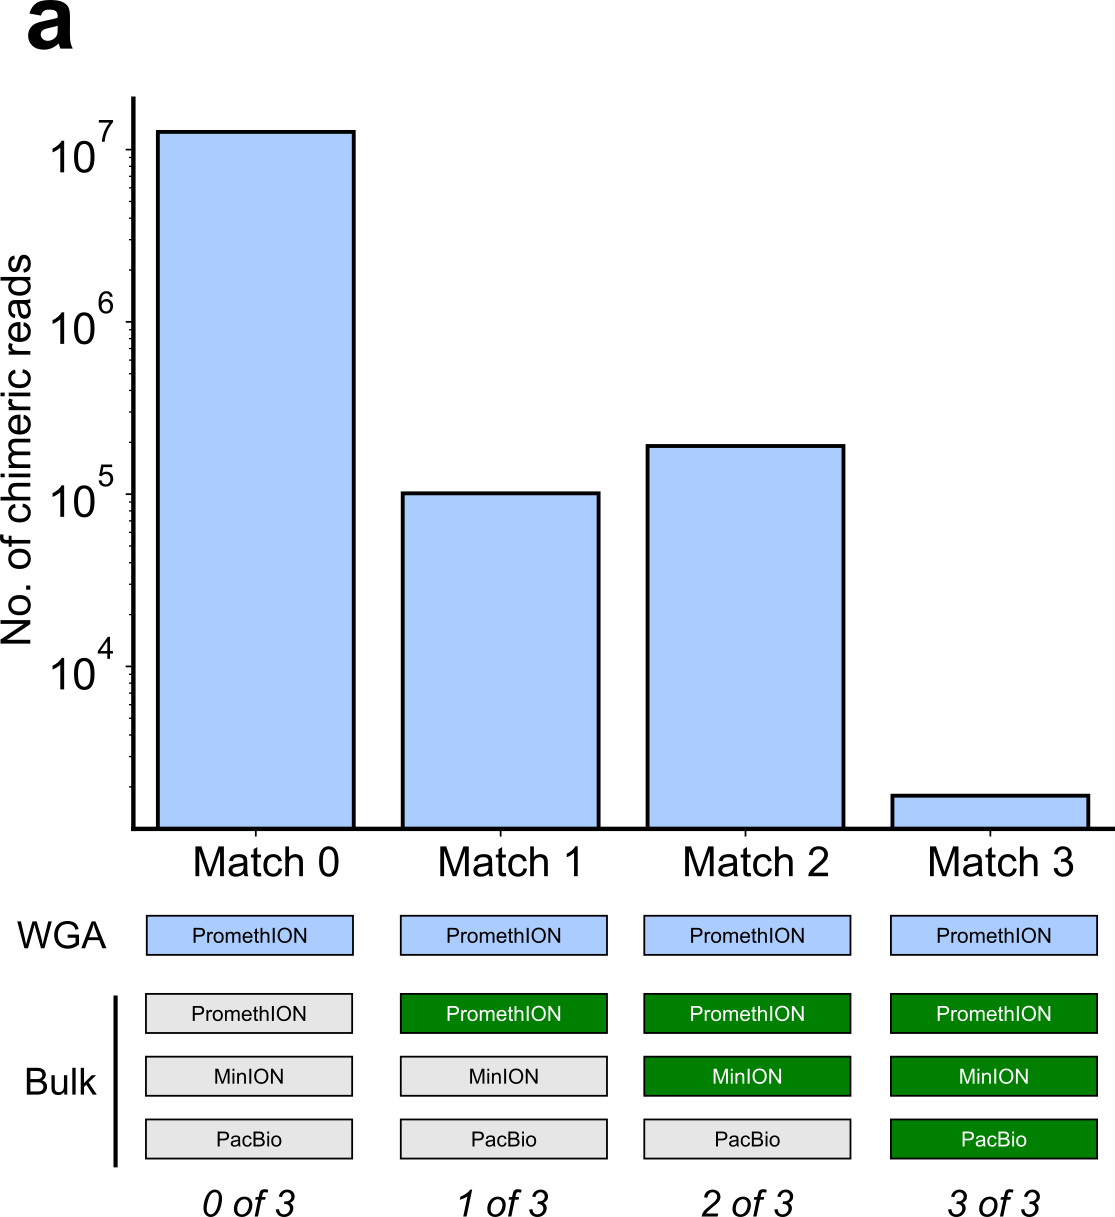
\includegraphics[width=0.8\textwidth]{final_figures/sf1}
	\end{center}
	\caption{{\bf Distribution of chimeric read matches between \gls{wga} and bulk sequencing datasets.}
		Bar chart showing the number of chimeric reads (y-axis, log scale) stratified by the number of matches found when comparing \gls{wga} chimeric reads against bulk sequencing data (x-axis). Match 0 indicates chimeric reads with no matches in bulk data (labeled as artificial chimeric artifacts, $\sim$10$^7$ reads). Match 1, 2, and 3 indicate chimeric reads with 1, 2, or 3 matches in bulk data respectively (labeled as biological reads, $\sim$10$^5$ reads each). This matching strategy forms the basis for ground truth labeling in supervised training.}\label{fig:sf1}
\end{figure}

% \begin{figure}[!ht]
% 	\begin{center}
% 		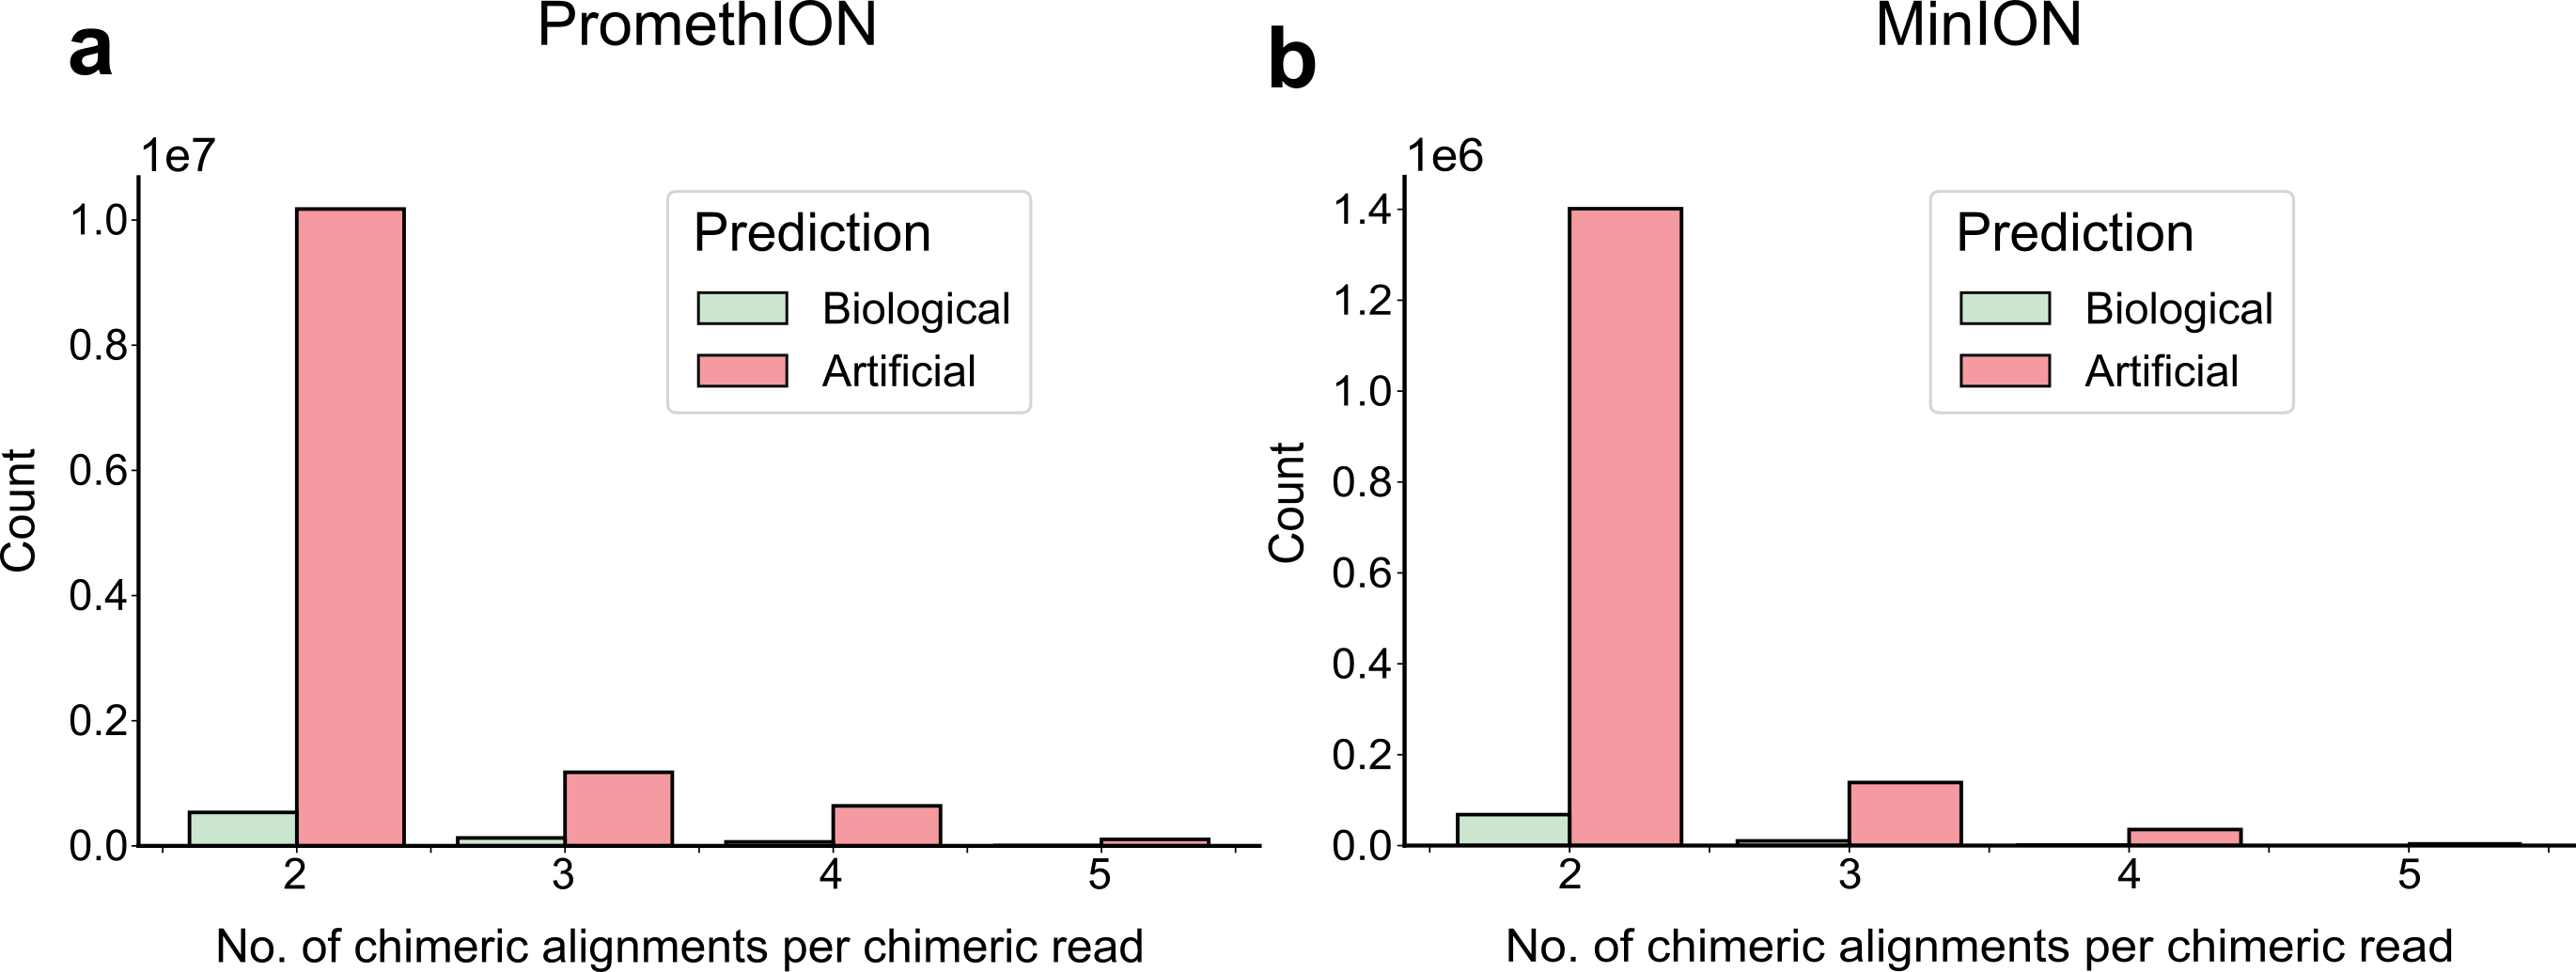
\includegraphics[width=\textwidth]{final_figures/sf2}
% 	\end{center}
% 	\caption{{\bf Distribution of chimeric alignments per chimeric read stratified by ChimeraLM prediction.}
% 		(a) PromethION P2 platform chimeric alignment analysis. Bar chart showing the distribution of chimeric reads based on the number of chimeric alignments per read (x-axis: 2, 3, 4+ alignments) and total read count (y-axis, log scale). Bars are colored by ChimeraLM's binary classification: biological (dark teal) and artificial (coral). Analysis includes only reads identified as chimeric (minimum 2 alignments per read).
% 		(b) MinION Mk1c platform chimeric alignment analysis. Bar chart showing the distribution of chimeric reads based on the number of chimeric alignments per read (x-axis: 2, 3, 4+ alignments) and total read count (y-axis, log scale). Bars are colored by ChimeraLM's binary classification: biological (dark teal) and artificial (coral). Analysis includes only reads identified as chimeric (minimum 2 alignments per read).}\label{fig:sf2}
% \end{figure}

\bmhead{Acknowledgements}

We thank Tingyou Wang for guidance on figure preparation.
This project was supported in part by NIH grants R35GM142441 and R01CA259388 awarded to RY.

\section*{Declarations}

\bmhead{Author Contributions}

YL, QG and RY designed the study.
YL and QG performed the analysis.
QG performed the experiments.
YL designed and implemented the model and computational tool.
YL, QG and RY wrote the manuscript.
RY supervised this work.

\bmhead{Data Availability}

\bmhead{Code Availability}

ChimeraLM, implemented in Python, is open source and available on GitHub (\url{https://github.com/ylab-hi/ChimeraLM}) under the Apache License, Version 2.0.
The package can be installed via PyPI (\url{https://pypi.org/project/chimeralm}) using pip, with wheel distributions provided for Windows, Linux, and macOS to ensure easy cross-platform installation.
An interactive demo is available on Hugging Face (\url{https://huggingface.co/spaces/yangliz5/chimeralm}), allowing users to test ChimeraLM's functionality without local installation.
For large-scale analyses, we recommend using ChimeraLM on systems with \gls{gpu} acceleration. Detailed system requirements and optimization guidelines are available in the repository's documentation.

\bmhead{Conflict of interest}

RY has served as an advisor/consultant for Tempus AI, Inc. This relationship is unrelated to and did not influence the research presented in this study.

% Some journals require declarations to be submitted in a standardised format. Please check the Instructions for Authors of the journal to which you are submitting to see if you need to complete this section. If yes, your manuscript must contain the following sections under the heading `Declarations':

% \begin{itemize}
% 	\item Funding
% 	\item Conflict of interest/Competing interests (check journal-specific guidelines for which heading to use)
% 	\item Ethics approval and consent to participate
% 	\item Consent for publication
% 	\item Data availability
% 	\item Materials availability
% 	\item Code availability
% 	\item Author contribution
% \end{itemize}
%
% \noindent
% If any of the sections are not relevant to your manuscript, please include the heading and write `Not applicable' for that section.

\begin{appendices}

	\printglossaries

	% \section{Section title of first appendix}\label{secA1}
	%
	% An appendix contains supplementary information that is not an essential part of the text itself but which may be helpful in providing a more comprehensive understanding of the research problem or it is information that is too cumbersome to be included in the body of the paper.
	%
	%%=============================================%%
	%% For submissions to Nature Portfolio Journals %%
	%% please use the heading ``Extended Data''.   %%
	%%=============================================%%

	%%=============================================================%%
	%% Sample for another appendix section			       %%
	%%=============================================================%%

	%% \section{Example of another appendix section}\label{secA2}%
	%% Appendices may be used for helpful, supporting or essential material that would otherwise
	%% clutter, break up or be distracting to the text. Appendices can consist of sections, figures,
	%% tables and equations etc.
\end{appendices}

%%===========================================================================================%%
%% If you are submitting to one of the Nature Portfolio journals, using the eJP submission   %%
%% system, please include the references within the manuscript file itself. You may do this  %%
%% by copying the reference list from your .bbl file, paste it into the main manuscript .tex %%
%% file, and delete the associated \verb+\bibliography+ commands.                            %%
%%===========================================================================================%%

\bibliography{clean}% common bib file
%% if required, the content of .bbl file can be included here once bbl is generated
%%\input sn-article.bbl

\end{document}
